\hypertarget{ux57faux4e8eux68afux5ea6ux4e0eux8d85ux7f51ux7edcux7684ux6301ux7eedux5b66ux4e60}{%
\chapter{基于梯度与超网络的持续学习}\label{ux57faux4e8eux68afux5ea6ux4e0eux8d85ux7f51ux7edcux7684ux6301ux7eedux5b66ux4e60}}

\hypertarget{ux57faux4e8eux5728ux7ebfux81eaux84b8ux998fux7684ux6301ux7eedux5b66ux4e60ux8bbaux6587}{%
\section{基于在线自蒸馏的持续学习（论文）}\label{ux57faux4e8eux5728ux7ebfux81eaux84b8ux998fux7684ux6301ux7eedux5b66ux4e60ux8bbaux6587}}

\begin{quote}
本文是论文阅读笔记，内容代表对应论文方法或作者理解，不应直接视为领域共识或工程最佳实践。
\end{quote}

\hypertarget{ux4e00ux81eaux84b8ux998fux7684ux63d0ux51faux80ccux666fux548cux6838ux5fc3ux539fux7406}{%
\subsection{一、自蒸馏的提出背景和核心原理}\label{ux4e00ux81eaux84b8ux998fux7684ux63d0ux51faux80ccux666fux548cux6838ux5fc3ux539fux7406}}

对于test-time的持续学习，很多场景无法定义RL的奖励函数，更不可能使用SFT。我们希望模型从自身的经验和环境反馈中自主学习。

自蒸馏策略优化（SDPO）提出，可以学生模型让仅根据原始的指令提示，自回归地生成一个尝试。当环境详细的反馈（如报错信息）后，权重相同的教师模型根据原始指令+环境反馈，利用强大的上下文学习能力，在学生模型生成序列的每个位置上，预测下一个词元的正确分布（根据看到的环境反馈得出反思，从而可以纠正学生的错误输出）。随后，更新学生模型的权重，让学生模型通过最小化 KL 散度 \(D_{\mathrm{KL}}(\pi_{\mathrm{student}}\Vert \pi_{\mathrm{teacher}})\) 来逼近这个分布：

\[
\begin{aligned}
\nabla_\theta D_{\mathrm{KL}}(\pi_\theta \Vert \pi)
&=
\sum_{v \in \mathcal{V}} \pi_\theta(v \mid y_{<t}) \nabla_\theta \log \pi_\theta(v \mid y_{<t})
\left(
\log \frac{\pi_\theta(v \mid y_{<t})}{\pi(v \mid y_{<t}, c)} + 1
\right)
\end{aligned}
\]

自蒸馏微调（SDFT）也让同一个模型在训练中同时扮演``教师''和``学生''两个角色。学生模型仅接收原始的任务提示词并自回归生成；教师模型接收任务提示词和专家演示，通过大模型的上下文学习能力，每次在学生模型的前 \(i-1\) 个 token 基础上生成包含正确任务意图的第 \(i\) 个 token 作为高质量指导信号，然后也用上面所述的反向KL散度。这里的``专家演示''未必要来自外部，也可以是自身根据后来改出的正确答案。可以类似人类在睡眠时巩固一样，和主进程异步地按自己对同一个问题后来得出的正确答案、优秀经验，对最初上下文较少时的错误输出进行纠正。

\hypertarget{ux4e8cux707eux96beux6027ux9057ux5fd8ux53caux5176ux89e3ux51b3ux65b9ux6848}{%
\subsection{二、``灾难性遗忘''及其解决方案}\label{ux4e8cux707eux96beux6027ux9057ux5fd8ux53caux5176ux89e3ux51b3ux65b9ux6848}}

\begin{enumerate}
\def\labelenumi{\arabic{enumi}.}
\tightlist
\item
  参数复位与记忆系统
\end{enumerate}

由于这种算法对于每个token都会产生梯度，用平均梯度批量更新，在持久化累加到大模型的全局参数上时，由于缺乏原始对齐数据或广泛预训练分布的正则化约束，优化器会迫使模型参数迅速滑向当前这道特定题目的局部最优解。随着高频次、碎片化的test-time任务不断冲刷，模型原本在训练中为了通用对话和广泛知识构建的参数流形就会被破坏，从而表现出严重的灾难性遗忘。故此方法在运用时仅限于对于特定任务的微调，任务结束后应当归位到原来的参数。

尽管参数需要归位，但我们仍然希望经验能被重新复用。我们可以将通过自蒸馏获得的经验记入记忆系统，通过类似RAG的方式，按需获取并注入上下文，从而既避免永久性修改参数本身导致的``灾难性遗忘''，又高效利用过程中留下的经验。

\begin{enumerate}
\def\labelenumi{\arabic{enumi}.}
\setcounter{enumi}{1}
\tightlist
\item
  旁路或限定微调模块
\end{enumerate}

可以不对全参数进行微调，如只在最后1/4的Transformer Block中的双层MLP/MoE中的一层进行微调；也可以引入LoRA，只在低维流形内修改，但若维度太小会导致不同方面的经验向量无法正交存储，在每个token都更新的高频更新下，会导致无法形成长期记忆。

\begin{enumerate}
\def\labelenumi{\arabic{enumi}.}
\setcounter{enumi}{2}
\tightlist
\item
  经验回放
\end{enumerate}

引入回放机制后，算法的工作流将演变为一个同时维护当前状态和过去记忆的动态系统：

\begin{enumerate}
\def\labelenumi{\arabic{enumi}.}
\tightlist
\item
  记忆缓冲区初始化与维护（Buffer Initialization）：
\end{enumerate}

在系统启动时，建立一个固定容量的记忆缓冲区 \(\mathcal{M}\)。其中预先存入少量代表全局数据分布的锚点数据，例如多样化的通用对话、基础逻辑问答。

\begin{enumerate}
\def\labelenumi{\arabic{enumi}.}
\setcounter{enumi}{1}
\tightlist
\item
  当前任务自蒸馏（Current Task Distillation）：
\end{enumerate}

当面临新的 Test-time 任务 \(x_{\mathrm{curr}}\) 时，模型进行自回归尝试、获取环境反馈，并由教师模型生成当前任务的理想分布 \(\pi_{\mathrm{teacher}}\)，即标准 SDFT/SDPO 流程。随后计算当前任务的局部损失 \(\mathcal{L}_{\mathrm{curr}}\)。

\begin{enumerate}
\def\labelenumi{\arabic{enumi}.}
\setcounter{enumi}{2}
\tightlist
\item
  记忆采样与混合计算（Replay Sampling \& Mixing）：
\end{enumerate}

从缓冲区 \(\mathcal{M}\) 中采样一小批历史经验集：

\[
\mathcal{B}_{\mathrm{replay}} = \left\{(x_i, y_i)\right\}_{i=1}^{k}
\]

在这些历史数据上计算模型的常规交叉熵损失，或保持之前预测概率的自蒸馏损失，记作 \(\mathcal{L}_{\mathrm{replay}}\)。

\begin{enumerate}
\def\labelenumi{\arabic{enumi}.}
\setcounter{enumi}{3}
\tightlist
\item
  联合梯度更新（Joint Gradient Update）：
\end{enumerate}

将当前任务损失与回放损失进行加权求和，然后执行反向传播更新全局参数 \(\theta\)：

\[
\theta \leftarrow \theta - \eta \nabla_\theta\left(\lambda \mathcal{L}_{\mathrm{curr}} + (1-\lambda)\mathcal{L}_{\mathrm{replay}}\right)
\]

\begin{enumerate}
\def\labelenumi{\arabic{enumi}.}
\setcounter{enumi}{4}
\tightlist
\item
  记忆动态更新（Dynamic Buffer Update）：
\end{enumerate}

当前任务解决后，评估该任务的价值，例如它是否修正了模型之前的一个重大错误，或者是否具有高``惊喜度'' Negative Log-Likelihood。如果价值极高，则将其提炼为 \((x_{\mathrm{curr}}, y_{\mathrm{correct}})\) 压入缓冲区 \(\mathcal{M}\)，并根据特定策略，例如水库采样或基于遗忘风险的剔除，替换掉一条旧记忆。

\hypertarget{ux4e09ux81eaux84b8ux998fux65b9ux6cd5ux7684ux7f3aux9677}{%
\subsection{三、自蒸馏方法的缺陷}\label{ux4e09ux81eaux84b8ux998fux65b9ux6cd5ux7684ux7f3aux9677}}

微软等的研究表明，尽管自蒸馏在化学问答、代码生成等任务中让模型取得了较大进步，但在具有长推理路径的复杂数学推理任务中，自蒸馏可能反而导致模型性能下降。根本原因在于自蒸馏抑制了模型内部标示不确定性假设的``认知不确定性表达''。这些词汇在生成序列中本来承担了不同的认知功能：

触发重估（如wait, actually）：通常表明模型在其计算图的当前路径上识别到了潜在的矛盾，准备回退或修改之前的假设。

扩展计算时间（如hmm）：作为填充词汇，为模型争取额外的自回归步骤，以便计算更复杂的潜在状态。

假设检验（如perhaps, maybe, seems, might, likely）：表示模型提出了一种可能的解法，但尚未赋予高置信度，从而在逻辑语义上保持开放性。

分支建立（如alternatively）：引入并行的推理路径进行对比评估。

验证机制（如check）：显式触发对中间结果的重新计算与核对。

在包含这些标记的推理轨迹中，模型具有更宽泛的容错空间。然而，当教师模型被赋予标准答案等高信息量上下文时，其生成的推理过程变得确定且简短，导致学生模型在蒸馏过程中盲目模仿这种高度自信的输出风格，去除了这些认知不确定性信号，模型往往会过早地将高概率权重分配给可能错误的假设，导致探索能力下降，陷入逻辑死胡同且无法自我修正。

\hypertarget{ux53c2ux8003ux6587ux732e-147}{%
\subsection{参考文献}\label{ux53c2ux8003ux6587ux732e-147}}

\begin{itemize}
\tightlist
\item
  Shenfeld, I., Damani, M., Hubotter, J., \& Agrawal, P. (2026). \href{https://arxiv.org/abs/2601.19897}{Self-Distillation Enables Continual Learning}. arXiv:2601.19897.
\item
  Hubotter, J., Lubeck, F., Behric, L., et al.~(2026). \href{https://arxiv.org/abs/2601.20802}{Reinforcement Learning via Self-Distillation}. arXiv:2601.20802.
\item
  Kim, J., Luo, X., Kim, M., et al.~(2026). \href{https://arxiv.org/abs/2603.24472}{Why Does Self-Distillation (Sometimes) Degrade the Reasoning Capability of LLMs?}. arXiv:2603.24472.
\end{itemize}

\clearpage

\hypertarget{ux90e8ux5206ux6743ux91cdux5c31ux5730ux66f4ux65b0ux7684tttux8bbaux6587}{%
\section{部分权重就地更新的TTT（论文）}\label{ux90e8ux5206ux6743ux91cdux5c31ux5730ux66f4ux65b0ux7684tttux8bbaux6587}}

\begin{quote}
本文是论文阅读笔记，内容代表对应论文方法或作者理解，不应直接视为领域共识或工程最佳实践。
\end{quote}

\hypertarget{ux4e00ttt-e2e}{%
\subsection{一、TTT-E2E}\label{ux4e00ttt-e2e}}

\hypertarget{ux4e00ux6838ux5fc3ux601dux60f3-13}{%
\subsubsection{（一）核心思想}\label{ux4e00ux6838ux5fc3ux601dux60f3-13}}

对于长上下文的处理，在实际生产中，重要的不是一字不落地记住所有细节，而是对上下文建构理解，并将其内化。TTT-End to End（TTT-E2E）提出可以在长上下文处理中，通过在推理时不断用Next token prediction实现持续学习；在训练时，也把目标替换为``进行若干步更新后表现最好''的元学习目标，而不是``冻结参数时开箱即用的表现''，以防止参数漂移、对异常片段的过拟合等。

\hypertarget{ux4e8cux6a21ux578bux67b6ux6784-2}{%
\subsubsection{（二）模型架构}\label{ux4e8cux6a21ux578bux67b6ux6784-2}}

在推理时，冻结嵌入层（Embedding）、归一化层和注意力层，只更新多层感知机（MLP）的权重，以避免外层循环的梯度不稳定。具体来说，只更新网络最后1/4的Transformer block中的第一个MLP层（为了防止TTT过程遗忘预训练知识，在被更新的block中，额外添加一个静态的第二MLP层作为预训练知识的``安全存储区''；前3/4的Transformer block起表征提取作用，故不动）。

\begin{enumerate}
\def\labelenumi{\arabic{enumi}.}
\tightlist
\item
  \textbf{测试时优化：内层循环（Inner Loop）}
\end{enumerate}

在测试阶段，模型接收到上下文后，并非直接一次性输出，而是先利用这些上下文进行自我更新。

\begin{itemize}
\tightlist
\item
  \textbf{基础架构}：模型基于标准 Transformer，但将全注意力替换为滑动窗口注意力（Sliding-Window Attention, SWA），窗口大小为 \(8K\)。
\item
  \textbf{Mini-Batch 更新规则}：为了提高并行性和稳定性，TTT 采用小批量更新。对于大小为 \(\hat b\) 的小批量，模型权重更新公式为：
\end{itemize}

\[
W_i = W_{i-1}
- \eta\frac{1}{\hat b}
\sum_{t=(i-1)\hat b+1}^{i\hat b}
\nabla l_t(W_{i-1})
\]

其中 \(l_t\) 是标准交叉熵损失函数：

\[
l_t(W)=CE(f(x_{t-1};W),x_t)
\]

\begin{enumerate}
\def\labelenumi{\arabic{enumi}.}
\setcounter{enumi}{1}
\tightlist
\item
  \textbf{训练时元学习：外层循环（Outer Loop）}
\end{enumerate}

如果模型在测试时需要为了测试时更新权重``做好准备''，直接进行 TTT 效果会很差。因此，在预训练阶段，作者使用元学习来寻找最优的初始权重 \(W_0\)。

\begin{itemize}
\tightlist
\item
  \textbf{端到端损失函数}：训练时的目标函数直接等于测试时经过 TTT 更新后的平均损失：
\end{itemize}

\[
\mathcal{L}(W_0;X)=
\frac{1}{T}\sum_{i=1}^{T/\hat b}\sum_{t=(i-1)\hat b+1}^{i\hat b}
l_t(W_{i-1})
\]

\begin{itemize}
\tightlist
\item
  \textbf{梯度反传}：外层循环通过对上述损失求 \(W_0\) 的梯度，即隐藏的梯度 \(\nabla\mathcal{L}(W_0)\)，来优化初始权重，使得模型天生就具备``在测试时快速学习''的能力。
\end{itemize}

\hypertarget{ux4e09ux7b97ux6cd5ux5de5ux4f5cux6d41}{%
\subsubsection{（三）算法工作流}\label{ux4e09ux7b97ux6cd5ux5de5ux4f5cux6d41}}

\begin{enumerate}
\def\labelenumi{\arabic{enumi}.}
\tightlist
\item
  \textbf{前向传播（Forward Pass）}：接收给定的上下文 token \(x_1\)。信号沿着向上的箭头逐层传播。首先经过底部的 embedding 层，然后穿过前 \(3L/4\) 个完全冻结的 Transformer 块（仅包含滑动窗口注意力和 MLP）。
\item
  \textbf{局部预测}：信号继续穿过顶部的 \(L/4\) 个 Transformer 块。在这部分块中，除了常规网络，还包含一个专门用于 TTT 更新的额外 MLP 层。最终在网络末端输出对下一个词的预测概率分布 \(\hat p_2\)。
\item
  \textbf{全局损失计算（Global Loss）}：当系统接收到真实的下一个上下文 token \(x_2\) 时，在网络的绝对顶端计算标准的交叉熵损失 \(l_2\)。
\item
  \textbf{误差反向传播（Backward Pass）}：图中的向下箭头代表梯度的反向传播。关键设计在于，梯度仅穿过最后 \(L/4\) 个网络块，并在向下传播到 \(3L/4\) 的边界处被截断。
\item
  \textbf{状态更新（State Update）}：利用截断的梯度，只更新被标为 TTT 的动态 MLP 层，其他网络参数保持冻结。
\item
  \textbf{循环与未来预测}：现在，将 \(x_2\) 作为新的输入，重复上述过程。被更新过的 MLP 使模型具备``记住前文''的能力，从而继续预测未来的 \(x_3\)。
\end{enumerate}

对比以Titans为代表的``K-V记忆''类Test time training方法：

\begin{enumerate}
\def\labelenumi{\arabic{enumi}.}
\tightlist
\item
  \textbf{逐层前向流动}：输入 \(x_1\) 经过 embedding 后，进入总共 \(L\) 个 Transformer 块的第 \(l\) 块，得到局部输入 \(x_1^{(l)}\)。
\item
  \textbf{键值投影（Key-Value Projection）}：在块内部，输入分别通过外层循环参数 \(\theta_K\) 和 \(\theta_V\) 进行线性投影，生成当前的 Key 和 Value。
\item
  \textbf{局部代理预测与损失计算}：该层内的 MLP 尝试根据 Key 来预测 Value，得到预测值 \(\hat l_1^{(l)}\)。随后，将真实 Value 与预测值之间的均方误差作为代理损失：
\end{enumerate}

\[
l^{(l)}_{\mathrm{TTT}}\left(W^{(l)}_{t-1}\right)
=
\left\|g\!\left(\theta_K^{(l)}x_t^{(l)};W^{(l)}_{t-1}\right)
- \theta_V^{(l)}x_t^{(l)}
\right\|^2
\]

\begin{enumerate}
\def\labelenumi{\arabic{enumi}.}
\setcounter{enumi}{3}
\tightlist
\item
  \textbf{局部状态更新}：图中的短向下箭头表示，梯度不会跨层流动。该层只在当前层内部反向传播，更新该层内部特殊 MLP 的权重。
\item
  \textbf{生成该层输出并传递}：当输入 \(x_2\) 到达该层得到 \(x_2^{(l)}\) 时，使用 \(\theta_K\) 投影后，送入更新后的蓝色 MLP，得到该层的最终输出 \(z_2^{(l)}\)，再传递给更上一层。
\item
  \textbf{顶层预测}：经过所有 \(L\) 层的局部更新和前向传递后，在顶层通过 Softmax 预测 \(\hat p_3\)。
\end{enumerate}

\begin{figure}[htbp]
\centering
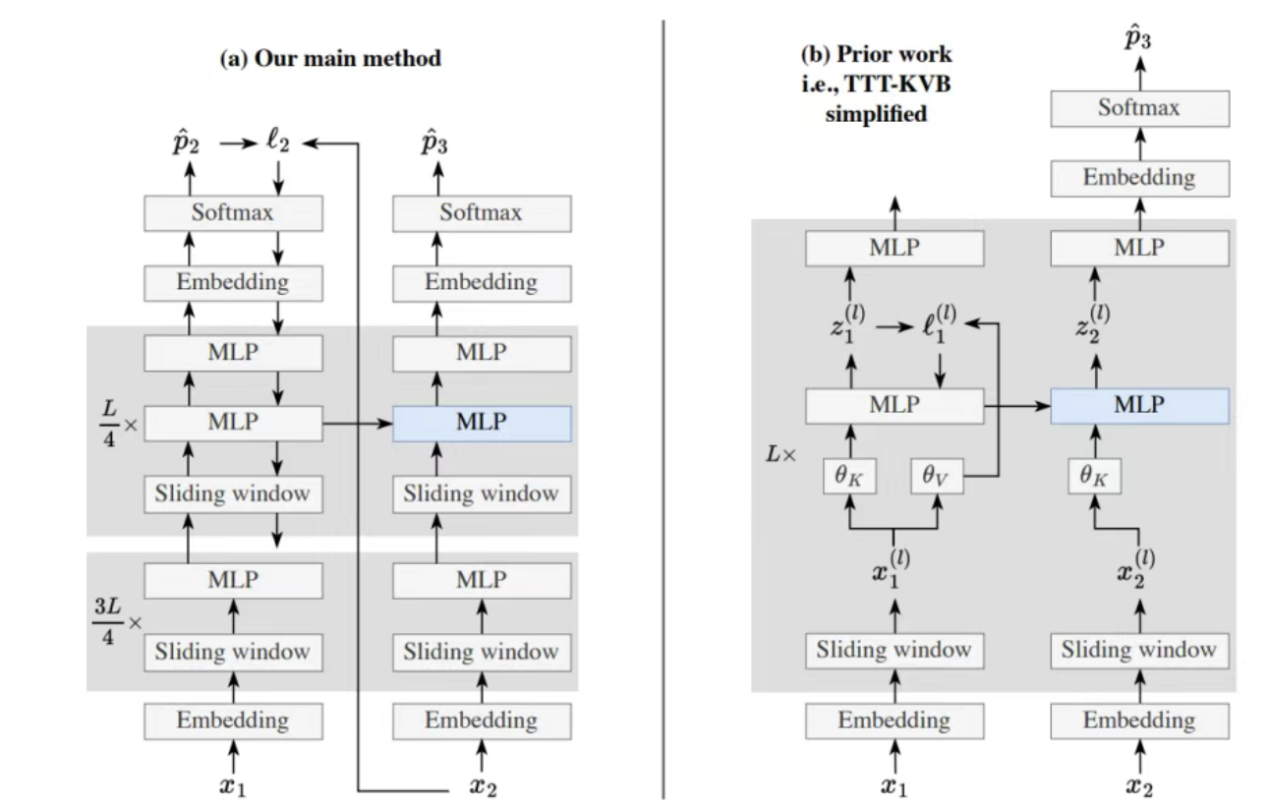
\includegraphics{images/image-0047.png}
\caption{TTT-E2E 与 TTT-KVB 的结构对比}
\end{figure}

\hypertarget{ux56dbux5982ux4f55ux907fux514dux5728ux663eux5b58ux4e2dux5b9eux4f8bux5316ux4e8cux9636hessianux77e9ux9635}{%
\subsubsection{（四）如何避免在显存中实例化二阶Hessian矩阵？}\label{ux56dbux5982ux4f55ux907fux514dux5728ux663eux5b58ux4e2dux5b9eux4f8bux5316ux4e8cux9636hessianux77e9ux9635}}

事实上，元学习的表达式中确实出现了二阶Hessian矩阵：

\[
\nabla_\theta J_{T_i}(\theta_i')
=
\nabla_{\theta_i'}J_{T_i}(\theta_i')
\cdot
\nabla_\theta\theta_i'
=
\nabla_{\theta_i'}J_{T_i}(\theta_i')
\cdot
\left(I+\alpha\nabla_\theta^2J_{T_i}(\theta)\right)
\]

但它是以和向量乘积的形式存在的，简化为考虑 Hessian 矩阵 \(H\) 和向量 \(v\) 乘积计算的问题：

\begin{enumerate}
\def\labelenumi{\arabic{enumi}.}
\tightlist
\item
  \textbf{计算一阶梯度}：对损失函数 \(\mathcal{L}\) 做一次常规反向传播，得到一阶梯度向量 \(g\)：
\end{enumerate}

\[
g=\nabla_\theta \mathcal{L}(\theta)
\]

此时显存开销为 \(O(N)\)，即存储梯度向量的大小。

\begin{enumerate}
\def\labelenumi{\arabic{enumi}.}
\setcounter{enumi}{1}
\tightlist
\item
  \textbf{构造标量点积}：将梯度向量 \(g\) 与目标向量 \(v\) 点积，得到纯标量：
\end{enumerate}

\[
S=g^\top v
\]

\begin{enumerate}
\def\labelenumi{\arabic{enumi}.}
\setcounter{enumi}{2}
\tightlist
\item
  \textbf{对标量求一阶导数}：对标量 \(S\) 再关于参数 \(\theta\) 求梯度：
\end{enumerate}

\[
\nabla_\theta S
= \nabla_\theta(g^\top v)
= (\nabla_\theta g)^\top v
= H v
\]

这一步实质上是在第一次反向传播建立的计算图上，再进行一次反向传播（reverse-over-reverse autodiff），显存开销仍保持在 \(O(N)\)。

这样的计算总开销约等于两次独立的前向+反向传播。

\hypertarget{ux4e94ux6838ux5fc3ux8ba1ux7b97ux5f00ux9500}{%
\subsubsection{（五）核心计算开销}\label{ux4e94ux6838ux5fc3ux8ba1ux7b97ux5f00ux9500}}

虽然单个时间步避免了 \(O(N^2)\) 的显存操作，但在 TTT-E2E 架构中，系统必须在长达数十万的 token 序列上展开计算图，这仍然引出了另一个维度的灾难。

\begin{enumerate}
\def\labelenumi{\arabic{enumi}.}
\tightlist
\item
  \textbf{随时间反向传播（BPTT）的状态膨胀}：
  在传统 RNN 或全注意力 Transformer 中，计算图随时间展开时，隐状态数量会随着序列长度线性增长。但在 TTT-E2E 的内层循环中，模型是将自身参数矩阵 \(W\) 作为随着时间演进的``隐状态''来进行持续学习，其内层更新规则类似于：
\end{enumerate}

\[
W_i = W_{i-1} - \eta\nabla_W l_i(W_{i-1})
\]

外层循环要计算 \(\nabla_{W_0}\mathcal{L}\)，必须穿过所有时间步反向传播：

\[
\frac{\partial\mathcal{L}}{\partial W_0}
=
\sum_i
\frac{\partial l_i}{\partial W_{i-1}}
\left(
\prod_{j=1}^{i-1}
\frac{\partial W_j}{\partial W_{j-1}}
\right)
\]

假设内层更新的 mini-batch 大小为 \(\hat b=1K\)，处理 \(T=128K\) 的上下文时，模型实际上要在内层循环中连续走 \(128\) 步梯度下降。

\begin{enumerate}
\def\labelenumi{\arabic{enumi}.}
\setcounter{enumi}{1}
\item
  \textbf{致命的显存耗尽（OOM）}：
  为了在反向传播时能计算上述梯度，前向传播必须在显存中保留所有中间状态。在 TTT 中，这意味着超长序列内每个下文切片都要形成一个巨大的权重链 \(W_1,W_2,\ldots,W_T\)，全部塞进显存。若不保存大部分中间权重，则反向传播时又需要重新计算，时间开销很大。
\item
  \textbf{``用时间换空间''的工程妥协：梯度检查点}：
  工程中可以用梯度检查点（Gradient Checkpointing）减少显存，但仍需要保存较多关键节点，并在反向传播时重新计算前向传播。对于 128K 级别的长上下文，这种方法仍会导致极高的时间成本。
\end{enumerate}

\hypertarget{ux516dux5173ux4e8emoe}{%
\subsubsection{（六）关于MoE}\label{ux516dux5173ux4e8emoe}}

正如前面所讨论的，TTT-E2E 能高效运行的核心在于把 1K 个 token 打包成一个 mini-batch，利用静态 MLP 计算统一的梯度 \(l_t(W)\) 并一次性更新。如果换成 MoE，这 \(1024\) 个 token 会被路由网络分配到不同专家：

\begin{itemize}
\tightlist
\item
  专家 A 可能只收到了 \(150\) 个 token 的梯度。
\item
  专家 B 可能收到了 \(300\) 个 token 的梯度。
\end{itemize}

底层 CUDA 算子无法对这些极其不规则的张量做 coalesced memory access，内存访问、线程排队、负载均衡都会变得困难。

MoE 的核心是门控（Gating）和路由网络，通常使用 Top-K 选择。这是一个不可导或至少高度非线性的过程。如果要在训练期让梯度穿过 TTT 更新步骤，再穿过 MoE 路由机制，其二阶导数的计算会变得不稳定，极易导致梯度爆炸或消失，模型根本无法收敛。

如果我们在架构设计上进行妥协，TTT-E2E 和 MoE 也并非完全不可结合。在 TTT-E2E 的官方实现中，为了保证速度，网络前 \(3/4\) 的层是\textbf{完全冻结（Frozen）}的，只有最后 \(1/4\) 的层参与 TTT 梯度更新。因此可行的折中方案是：

\begin{itemize}
\tightlist
\item
  \textbf{前 \(3/4\) 的冻结层使用 MoE 架构}：在这里发挥 MoE 的特长，用极低推理算力调用海量参数。
\item
  \textbf{后 \(1/4\) 的 TTT 层使用稠密（Dense）标准 MLP}：在这里保持规则的 dense 矩阵结构，使 TTT 更新具备高吞吐和稳定性。
\end{itemize}

\hypertarget{ux4e03ux5173ux4e8eux63a8ux7406ux548cagentux80fdux529b}{%
\subsubsection{（七）关于推理和Agent能力}\label{ux4e03ux5173ux4e8eux63a8ux7406ux548cagentux80fdux529b}}

Next-token prediction本质上是一种无监督的行为克隆。如果在测试时，强行让模型去拟合一段带有噪声、逻辑跳跃或次优决策的外部Context，确实极易引发``灾难性遗忘''，破坏掉前期通过PPO、GRPO等强化学习算法精调出的长链条推理和任务执行策略。

一种方法时让模型在测试时不去拟合外部给定的 Prompt，而是先利用现有的RL能力生成（或基于其他方法搜索出）高质量的推理步骤，然后结合环境反馈或验证对其经过筛选，利用经过筛选和重述的自身高质量数据来进行对前文所述的MLP模块的TTT更新，这就更类似于后面会提到的自蒸馏方法。

\hypertarget{ux4e8cin-place-ttt}{%
\subsection{二、In-Place TTT}\label{ux4e8cin-place-ttt}}

\hypertarget{ux4e00ux73b0ux6709ux6d4bux8bd5ux65f6ux8badux7ec3tttux65b9ux6cd5ux7684ux95eeux9898}{%
\subsubsection{（一）现有测试时训练（TTT）方法的问题}\label{ux4e00ux73b0ux6709ux6d4bux8bd5ux65f6ux8badux7ec3tttux65b9ux6cd5ux7684ux95eeux9898}}

\begin{enumerate}
\def\labelenumi{\arabic{enumi}.}
\item
  架构不兼容：现有TTT方法往往需要设计全新的独立层来替代自注意力机制，这意味着必须从头开始进行高昂的预训练，无法直接利用现有的模型。
\item
  计算效率低下：传统的TTT需要逐个Token顺序更新状态，严重限制了现代GPU/TPU的并行计算吞吐量。
\item
  目标不契合：以往TTT的自监督目标通常是简单的``重建当前词''，这与自回归语言模型``预测下一个词''的终极目标不一致。
\end{enumerate}

\hypertarget{ux4e8cux6838ux5fc3ux67b6ux6784-2}{%
\subsubsection{（二）核心架构}\label{ux4e8cux6838ux5fc3ux67b6ux6784-2}}

为解决上述问题，字节Seed提出了In-Place Test-Time Training框架。该框架不引入全新的网络层，而是直接将Transformer架构中普遍存在的MLP块中的最后一个投影矩阵 \(W_{\mathrm{down}}\) 征用为``快速权重''。这种``即插即用''的设计无需修改原始架构，保留了预训练权重的完整性，仅需极低的成本进行持续微调即可生效。

由于该方法作用于MLP层并与注意力机制互补，它允许以较大的分块为单位进行并行更新，极大地提升了在现代硬件上的吞吐量。

\hypertarget{ux4e09ux635fux5931ux51fdux6570}{%
\subsubsection{（三）损失函数}\label{ux4e09ux635fux5931ux51fdux6570}}

作者通过以下公式构造了一个带有``未来信息''的目标值 \(\hat V\)：

\[
V = \mathrm{Conv1D}(X_0)W_{\mathrm{target}}
\]

\begin{itemize}
\tightlist
\item
  \(X_0\) 是输入 token 最原始的词嵌入向量。
\item
  \(\mathrm{Conv1D}(\cdot)\) 是一个一维卷积。它以 3 层引入``未来信息''的核心机制，通过控制卷积核的权重，可以像滑动窗口一样把后面的词拉取过来。
\item
  \(W_{\mathrm{target}}\) 是一个可训练的矩阵，负责将卷积提取到的未来特征映射到合适的维度空间。
\end{itemize}

简单来说，我们希望神经网络最后一层的输出接近这个 \(V\) 值。神经网络最后一层的输出是上一层激活值 \(Z\) 经过权重 \(W_{\mathrm{down}}\) 后得到的。这里预测的词可以是上下文中的任何词，无论由用户、环境输入还是模型生成。

计算损失函数的过程如下：

\begin{enumerate}
\def\labelenumi{\arabic{enumi}.}
\tightlist
\item
  \textbf{计算当前输出}：模型使用当前的快速权重 \(W_{\mathrm{down}}^{(i)}\) 来处理当前激活值 \(Z_{[i]}\)，得到输出结果 \(O_{[i]}\)：
\end{enumerate}

\[
O_{[i]} = Z_{[i]}\left(W_{\mathrm{down}}^{(i)}\right)^T
\]

\begin{enumerate}
\def\labelenumi{\arabic{enumi}.}
\setcounter{enumi}{1}
\tightlist
\item
  \textbf{生成对齐目标}：模型利用 \(W_{\mathrm{target}}\) 计算出包含未来信息的标准答案 \(\hat V_{[i]}\)。
\item
  \textbf{计算损失并更新}：论文定义损失函数为两者之间的负内积：
\end{enumerate}

\[
\mathcal{L}=-\langle O_{[i]},\hat V_{[i]}\rangle_F
=
-\left\langle Z_{[i]}\left(W_{\mathrm{down}}^{(i)}\right)^T,\hat V_{[i]}\right\rangle_F
\]

最小化该负损失等价于最大化 \(Z_{[i]}(W_{\mathrm{down}})^\top\) 与 \(\hat V_{[i]}\) 之间的相似度。经过 \(W_{\mathrm{down}}\) 投影出来的结果如果能够与包含未来预测信息的 \(\hat V\) 高度对齐，说明该更新方向有效。

该方法采用极简的一阶更新。因为使用了最简单的内积作为损失函数，它的梯度推导清晰，快速权重更新为：

\[
W_{\mathrm{down}}^{(i)}
=
W_{\mathrm{down}}^{(i-1)}
+ \eta \hat V_{[i]}^\top Z_{[i]}
\]

为了防止 token 越来越多导致权重数值无界增长，论文还引入了 Frobenius 范数裁剪：

\[
\Delta W_{\mathrm{down}}^{(i)}
\leftarrow
\frac{\Delta W_{\mathrm{down}}^{(i)}}{\|\Delta W_{\mathrm{down}}^{(i)}\|_F}
\]

拓展：为什么不用交叉熵？

\begin{enumerate}
\def\labelenumi{\arabic{enumi}.}
\tightlist
\item
  Softmax的计算开销
\end{enumerate}

交叉熵路径中，模型必须把当前 \(d_{\mathrm{model}}\) 维隐状态映射到整个词表空间，词表大小可能达到 \(50K\) 到 \(150K\)。然后执行 Softmax、计算概率分布、求出误差，再反向传播穿过 LM Head 回到 MLP 层。TTT 的现实环境通常是推理阶段动态运行，如果每处理一个 chunk 都要做一次词表级别的反向传播，计算开销和显存占用都非常高。

\begin{enumerate}
\def\labelenumi{\arabic{enumi}.}
\setcounter{enumi}{1}
\tightlist
\item
  梯度公式简洁，易于优化
\end{enumerate}

如果采用非线性 Softmax 产生的高维非线性梯度，需要依赖深度学习框架进行 Top-K 内的大段反向图推导。而内积损失 \(C=-(ZW_{\mathrm{down}}^\top)\hat V^\top\) 的梯度对 \(W_{\mathrm{down}}\) 只有极其简单的解析解，避免了大规模反向图的维护和计算。

\begin{enumerate}
\def\labelenumi{\arabic{enumi}.}
\setcounter{enumi}{2}
\tightlist
\item
  上下文并行的要求
\end{enumerate}

为了实现计算加速，引入了上下文并行机制，利用并行扫描（Parallel Scan / Prefix Sum）来同时处理多个文本块。交叉熵的依赖链中，每一个 token 的分类都需要经过庞大的词表块，而内积损失对每个块而言只依赖于局部的 \(Z\)、目标 \(\hat V\) 和快速权重，梯度天然可以用矩阵加法/乘法组合，从而更容易并行化。

\hypertarget{ux56dbux4e3aux4ec0ux4e48ux5bf9ux63a8ux7406ux80fdux529bux7684ux5f71ux54cdux4e0dux5927}{%
\subsubsection{（四）为什么对推理能力的影响不大？}\label{ux56dbux4e3aux4ec0ux4e48ux5bf9ux63a8ux7406ux80fdux529bux7684ux5f71ux54cdux4e0dux5927}}

\begin{enumerate}
\def\labelenumi{\arabic{enumi}.}
\tightlist
\item
  架构层面
\end{enumerate}

In-Place TTT 并没有更新模型所有权重，而是做了一个非常精妙的隔离设计：

\begin{itemize}
\tightlist
\item
  \textbf{冻结``通用推理基座''}：模型的核心自注意力机制，以及 MLP 中间的 \(W_{\mathrm{up}}\) 和 \(W_{\mathrm{gate}}\) 都被完全冻结。作为``慢权重（Slow Weights）''保留了预训练阶段学到的常识逻辑和 agent 规划能力。
\item
  \textbf{只更新残差连接的一部分}：它仅将 MLP 的最后一个投影矩阵 \(W_{\mathrm{down}}\) 作为可热插拔更新模块。快速权重发生改变时，它实际上是在模型原有大推理路径之上做局部增量特征叠加：
\end{itemize}

\[
H_{\mathrm{out}} = H_{\mathrm{in}} + \mathrm{MLP}(H_{\mathrm{in}})
\]

当 \(W_{\mathrm{down}}\) 发生改变时，它主要是在原有完整推理路径之上增加一段局部记忆增强，不会破坏底层推理能力。

\begin{enumerate}
\def\labelenumi{\arabic{enumi}.}
\setcounter{enumi}{1}
\tightlist
\item
  目标函数层面
\end{enumerate}

论文指出，在实际工程实现中，这个目标函数并没有局限于单一的下一个 token。

\begin{itemize}
\tightlist
\item
  \textbf{局部未来特征的融合}：通过一维卷积 Conv1D 和映射矩阵 \(W_{\mathrm{target}}\) 的可学习组合，目标值 \(\hat V\) 实际上捕获的是一个局部未来 token 组合信息。
\item
  \textbf{与 MTP 思想相似}：这种设计与多 token 预测思路一致。强制模型在隐空间内一次性预测未来的多个演化状态，不仅不会削弱，反而会促进模型进行更深层的前向隐式规划。
\end{itemize}

\hypertarget{ux4e94ux9884ux586bux5145ux9636ux6bb5ux7684ux52a0ux901fux673aux5236ux56e0ux679cux586bux5145}{%
\subsubsection{（五）预填充阶段的加速机制：因果填充}\label{ux4e94ux9884ux586bux5145ux9636ux6bb5ux7684ux52a0ux901fux673aux5236ux56e0ux679cux586bux5145}}

在Agent任务中，模型需要在预填充阶段从长上下文中学习。

为了在预填充阶段进行高效训练，In-Place TTT 采用上下文并行（Context Parallelism），将极长的序列切分为多个块（chunk），并让所有 chunk 同时进行各自参数更新量 \(\Delta W\)。

这带来一个严重问题：理论上论文是为了``预测未来词''，如果在计算 chunk \(i\) 最后一个 token 的目标值 \(\hat V\) 时，卷积很有可能看到了哪怕一个未来的词，它就会跨界提取到 chunk \(i+1\) 的数据。这样就违反了跨块的数据依赖，chunk \(i\) 必须等待 chunk \(i+1\) 的数据，并行扫描算法的基石就会崩塌。

为确保对 chunk \(i\) 的更新量完全不包含未来的信息，作者在生成目标值时对 1D 卷积强行应用了因果填充：

\begin{itemize}
\tightlist
\item
  \textbf{常规卷积的视野}：如果卷积核大小为 \(5\)（即 \(K=5\)），为了计算位置 \(t\) 的特征，通常会取 \([t-2,t-1,t,t+1,t+2]\)，这显然包含了未来的信息。
\item
  \textbf{因果填充的具体做法}：实现中采用了核大小为 \(5\) 且带有因果填充的深度一维卷积。它会在序列左侧手动填充 \(4\) 个 \(0\)。这样一来，在计算位置 \(t\) 的特征时，感受野会变为 \([t-4,t-3,t-2,t-1,t]\)。
\end{itemize}

通过这种单向约束，每个 chunk 的计算被严格隔离在自己的边界内。这种局部机制使得高度并行的扫描算法在数学上完全等价于严格的因果序列过程。

当然，解码阶段仍然逐词串行输出和更新权重：

\begin{itemize}
\tightlist
\item
  \textbf{Apply}：模型直接使用当前维持的 \(W_{\mathrm{down}}\) 对这个 token 进行投影，得到输出。
\item
  \textbf{Update}：计算这个 token 带来的较小梯度增量 \(\Delta W\)，并将其累加到 \(W_{\mathrm{down}}\) 中。在这个过程中同样受到很小阈值 \(\tau=10^{-5}\) 的强制裁断保护，防止持续累积退化。
\end{itemize}

\hypertarget{ux53c2ux8003ux6587ux732e-148}{%
\subsection{参考文献}\label{ux53c2ux8003ux6587ux732e-148}}

\begin{itemize}
\tightlist
\item
  Tandon, A., Dalal, K., Li, X., et al.~(2025). \href{https://arxiv.org/abs/2512.23675}{End-to-End Test-Time Training for Long Context}. arXiv:2512.23675.
\item
  Feng, G., Luo, S., Hua, K., et al.~(2026). \href{https://arxiv.org/abs/2604.06169}{In-Place Test-Time Training}. arXiv:2604.06169.
\end{itemize}

\clearpage

\hypertarget{titansux4e0enested-learningux8bbaux6587}{%
\section{Titans与Nested Learning（论文）}\label{titansux4e0enested-learningux8bbaux6587}}

\begin{quote}
本文是论文阅读笔记，内容代表对应论文方法或作者理解，不应直接视为领域共识或工程最佳实践。
\end{quote}

\hypertarget{ux4e00titans}{%
\subsection{一、Titans}\label{ux4e00titans}}

Google Research提出的Titans将模型视为一个具有不同层次记忆系统的智能体，通过对Delta Attention进行泛化，引入了一种能够在测试时改变权重、进行记忆的长短期神经记忆模块。

\hypertarget{ux4e00ux6838ux5fc3ux601dux60f3-14}{%
\subsubsection{（一）核心思想}\label{ux4e00ux6838ux5fc3ux601dux60f3-14}}

Titans架构由三个相互关联的Hyper-heads组成，模拟了人类大脑处理信息的不同方式：

Transformer模块：类似于人类的短期记忆（工作记忆），负责处理当前数据流，通常使用窗口有限的注意力机制实现。

长期记忆模块：类似于人类的长期记忆，维护大小恒定的MLP，在推理过程中通过梯度下降不断更新其中的参数，从而``存储''长期的历史信息。

静态参数模块：训练后``冻结''的参数，存储全局知识和能力。

\hypertarget{ux4e8cux957fux671fux8bb0ux5fc6ux6a21ux5757ux7684ux57faux672cux539fux7406}{%
\subsubsection{（二）长期记忆模块的基本原理}\label{ux4e8cux957fux671fux8bb0ux5fc6ux6a21ux5757ux7684ux57faux672cux539fux7406}}

和Kimi Delta Attention类似，计算新信息的Key经过记忆模块后的输出与Value之间的误差，作为``惊讶度''，损失函数为：

\[
\mathcal{L}_{\Delta} = \frac{1}{2}\left\|S^\top k_t - v_t\right\|_2^2
\]

即梯度更新的幅度与误差成正比，误差大意味着过往信息中没有这部分内容，记忆模块通过梯度更新将其``记住''。

但Titans也作出了改进和泛化：

\begin{enumerate}
\def\labelenumi{\arabic{enumi}.}
\item
  将单一矩阵（线性层）改为MLP，包含了非线性激活函数。多层 MLP 的非线性表达能力远强于线性矩阵，能把更复杂的历史抽象压缩进参数里。
\item
  采用了动量法，原来的 MLP 为 \(\mathcal{M}_{t-1}\) 时，利用梯度的移动平均 \(S_t\) 更新 MLP 的参数：
\end{enumerate}

\[
\mathcal{M}_t = \mathcal{M}_{t-1} - \eta \nabla \mathcal{L}(\mathcal{M}_{t-1})
\]

这样可以增加前后token之间语境的连贯性。

需要注意的是，对于第 \(t\) 个输入 token（或段落，段落中的 token 并行经过记忆模块和推理，此时记忆模块记录上一段落及更早的记忆，即每段只用和原来之间的平均损失更新一次）检索时，输出一个由和输入段落同样多的 embedding 向量构成的序列（矩阵）：

\[
h_t = \mathcal{M}^{*}_{t-1}(q_t)
\]

上面所述的更新过程均发生在这步计算完成之后，因为记忆模块的目的是``检索过去的信息''，不能让本token的Key和Value混入其中影响判断。

\hypertarget{ux4e09ux8bb0ux5fc6ux6a21ux5757ux878dux5165ux6a21ux578bux67b6ux6784ux7684ux65b9ux5f0f}{%
\subsubsection{（三）记忆模块融入模型架构的方式}\label{ux4e09ux8bb0ux5fc6ux6a21ux5757ux878dux5165ux6a21ux578bux67b6ux6784ux7684ux65b9ux5f0f}}

Memory As a Context：将记忆检索结果作为上下文拼接，在处理长程依赖时表现最好。

Memory As a Gate：记忆与注意力分支并行并门控融合。

Memory As a Layer：记忆模块作为独立层顺序堆叠。效率最高但性能较差。这种顺序设计限制了模型同时利用注意力和神经记忆互补处理数据的能力，但优势在于能更好地适配FlashAttention等硬件加速技术。

\hypertarget{ux56dbux4e3aux4ec0ux4e48titansux65e0ux6cd5ux50cfkimi-delta-attentionux90a3ux6837ux8fc5ux901fux6295ux5165ux4e1aux754cux5e94ux7528}{%
\subsubsection{（四）为什么Titans无法像Kimi Delta Attention那样迅速投入业界应用？}\label{ux56dbux4e3aux4ec0ux4e48titansux65e0ux6cd5ux50cfkimi-delta-attentionux90a3ux6837ux8fc5ux901fux6295ux5165ux4e1aux754cux5e94ux7528}}

\begin{enumerate}
\def\labelenumi{\arabic{enumi}.}
\tightlist
\item
  必须保留计算图和显式执行反向传播
\end{enumerate}

核心在于上述的梯度表达式。Kimi Delta Attention之所以不需要显式执行反向传播，是因为其隐状态更新公式可直接求出解析解，通过矩阵乘法和加法来更新隐状态：

\[
\mathcal{M}_t = (1 - \alpha_t)\mathcal{M}_{t-1} + S_t
\]

\[
S_t = \eta_t S_{t-1} - \theta_t \nabla \mathcal{L}(\mathcal{M}_{t-1}; x_t)
\]

从而我们不需要保留计算图。

但是Titans存在非线性激活函数，其梯度在跨越激活函数的过程中，无法简单地写成解析闭式解，因此在推理更新阶段，系统必须维护一个针对该MLP模块的局部计算图来执行梯度下降，还要保留优化器状态。这带来了巨大的计算开销，和现在业界的推理优化方式不兼容。

【注意】Titans在训练时直接舍弃二阶梯度项，即训练时直接由L对``当前时刻的瞬时权重''求梯度。主要计算开销在于推理时的反向传播。

\begin{enumerate}
\def\labelenumi{\arabic{enumi}.}
\setcounter{enumi}{1}
\tightlist
\item
  Memory as a Context和Memory As a Gate无法用Flash Attention大规模并行
\end{enumerate}

我们知道，当输入第 \(t\) 个 token（或段落，段落中的 token 并行经过记忆模块和推理，此时记忆模块记录上一段落及更早的记忆，即每段只用和原来之间的平均损失更新一次）时，会先经过记忆模块：

\[
S_t = S_{t-1} + \beta_t k_t \left(v_t^\top - k_t^\top S_{t-1}\right)
\]

随后记忆模块更新：

\[
\mathcal{M}_t = (1 - \alpha_t)\mathcal{M}_{t-1} + S_t
\]

\[
S_t = \eta_t S_{t-1} - \theta_t \nabla \mathcal{L}(\mathcal{M}_{t-1}; x_t)
\]

MAC：处理第 2 段 \(q_2\)（\(x_2\)）就必须要先算出整个 \(\mathcal{M}_1\)，\(\mathcal{M}_1\) 需要通过 \(x_1\) 的值由梯度下降（无法写成显式解，即矩阵加法和乘法形式）才得到，必须一步一步串行。Flash Attention能在同一段上下文内部执行分块加速，但它无法跨段落融合。因为在算子层面，全局计算图被``权重更新''这一步骤物理性地切断了。

MAG：注意力分支中，对于一篇文章的各个段落（从1到t）可以完美使用Flash Attention。然而，由于最终输出需要注意力输出与记忆输出在每一位置进行门控融合，这限制了某些深度端到端的内核优化，因为数据必须从SRAM回写到HBM进行融合。

MAL：当所有段落都经过记忆层后，就完全同步了，可以直接用Flash Attention对整个文本的计算进行分块加速。

\hypertarget{ux4e94ux4e3aux4ec0ux4e48titansux5f3aux4e8eux7528ragux6ce8ux5165ux4e0aux4e0bux6587}{%
\subsubsection{（五）为什么Titans强于用RAG注入上下文？}\label{ux4e94ux4e3aux4ec0ux4e48titansux5f3aux4e8eux7528ragux6ce8ux5165ux4e0aux4e0bux6587}}

\begin{enumerate}
\def\labelenumi{\arabic{enumi}.}
\item
  压缩和抽象：简单地将文本块存入文件系统或向量数据库，检索出来的是原始数据。原始数据往往包含大量噪声，且没有经过``理解''和``压缩''。而Titans长期记忆模块通过梯度下降学习的是数据的抽象，它将成千上万个token的逻辑关系``浓缩''进神经网络的参数中。
\item
  ``惊讶度''驱动：只有当输入的信息违反了模型的预期（即很``令人惊讶''）时，模型才会产生强烈的梯度去大幅修改权重。这种机制让模型能自主决定哪些信息是真正值得``刻骨铭心''的，哪些只是重复的废话。
\item
  表达能力：大多数外置记忆检索基于线性相似度，且把序列切成块存进文件系统，块与块之间的逻辑流动会断裂；Titans使用深度（≥2层）MLP，且运用动量法使得前后token更连贯。
\item
  解决``迷失在中间''和窗口限制：RAG 提取回来的上下文依然受限于Transformer的窗口大小，且模型往往会产生``迷失在中间''的现象，无法有效利用极长的上下文；Titans是在参数层面更新，可以轻松扩展到更长的上下文窗口，而传统的检索或简单的循环模型此时性能会剧烈下滑。
\end{enumerate}

\hypertarget{ux516dux8badux7ec3ux65f6ux4e00ux9636ux9012ux5f52ux7684ux65f6ux95f4ux590dux6742ux5ea6}{%
\subsubsection{（六）训练时一阶递归的时间复杂度}\label{ux516dux8badux7ec3ux65f6ux4e00ux9636ux9012ux5f52ux7684ux65f6ux95f4ux590dux6742ux5ea6}}

在同一个块内，通过固定初始权重，可以一次性并行算出所有 token 的梯度项总和，时间复杂度为 \(O(1)\)。而在不同块间，训练时利用 \(S_0\) 算出 \(S_N\) 的时间复杂度是 \(O(\log N)\) 而非 \(O(N)\)。关键在于下一段对上一段的依赖关系可以写成一阶仿射递推。

Titans 中的动量项可以抽象为：

\[
S_t = \eta_t S_{t-1} + u'_t
\]

其中 \(u'_t=-\theta_t\nabla\mathcal{L}\)，即当前块带来的梯度更新项。进一步抽象为：

\[
S_t = a_t S_{t-1}+b_t
\]

其中 \(a_t=\eta_t\)，\(b_t=u'_t\)。若以二次损失为例，记忆矩阵也可写成同类线性变换：

\[
\mathcal{M}_t
=
\mathcal{M}_{t-1}(I-2\eta k_tk_t^\top)
 + 2\eta v_tk_t^\top
\]

也就是说，和Kimi Delta Attention一样，上式可看成对上一时刻记忆模块的线性变换。定义一个元组算子：

\[
\mathcal{T}_t=(a_t,b_t)
\]

它表示从状态 \(t-1\) 到状态 \(t\) 的转换。若有连续的两个转换 \(\mathcal{T}_1=(a_1,b_1)\) 与 \(\mathcal{T}_2=(a_2,b_2)\)，则合成后：

\[
S_2 = a_2(a_1S_0+b_1)+b_2
= (a_2a_1)S_0+(a_2b_1+b_2)
\]

利用 \(S_0\) 算出 \(S_2\)，只需要经过两个算子的融合：

\[
\mathcal{T}_{1:2}=(a_2a_1,\;a_2b_1+b_2)
\]

这种算子组合满足结合律：

\[
(\mathcal{T}_1\oplus\mathcal{T}_2)\oplus\mathcal{T}_3
=
\mathcal{T}_1\oplus(\mathcal{T}_2\oplus\mathcal{T}_3)
\]

由于满足结合律，就可以做并行扫描：

\begin{enumerate}
\def\labelenumi{\arabic{enumi}.}
\tightlist
\item
  第一层并行计算 \((1\oplus2)\)、\((3\oplus4)\)、\((5\oplus6)\ldots\)，每个单位时间消耗 1 个时间步。
\item
  第二层并行合并更长片段，得到 \((1-4)\)、\((5-8)\ldots\)。
\item
  对数层级地合并，经过 \(\log_2 N\) 次合并后即可得到从起始点到任意位置 \(t\) 的总转换算子。
\end{enumerate}

\hypertarget{ux4e8cnested-learning}{%
\subsection{二、Nested Learning}\label{ux4e8cnested-learning}}

\hypertarget{ux4e00ux95eeux9898ux80ccux666f-3}{%
\subsubsection{（一）问题背景}\label{ux4e00ux95eeux9898ux80ccux666f-3}}

无论是训练MLP还是运行Linear Attention，都可以被写成同一个通用的联想记忆优化目标：

\[
\mathcal{M}_{new}
=
\arg\min_{\mathcal{M}}
\mathrm{Mapping}(\mathrm{Key}, \mathrm{Value})
 + \mathrm{Regularization}
\]

MLP 训练是在低频（整个预训练数据集上、只训练一次）求解一个优化问题，将``输入 \(x\)''映射到``梯度信号 \(u\)''；Attention 推理是在高频（当前上下文窗口内、每次输入 token 时）求解一个优化问题，将``Key''线性回归映射到``Value''。也就是说，MLP的``训练''和 Attention 的``推理''，在数学形式上是完全一样的（都是在做梯度下降），区别仅仅在于它们的更新频率和数据来源不同。

现在的Transformer，本质是在外层MLP内部嵌入一个Attention层。进一步说，Transformer 实际上是一组并行的、频率不同的线性层，有的线性层（MLP）更新得很慢（由于预训练），有的线性层（Attention）更新得极快（在推理时实时更新）。

外层是一个极低频优化的MLP，它在预训练时注入通用知识，并永久记忆，但无法更新（更新频率为0）；内层则是一个高频优化的线性回归，它（在任务结束前）每输入一个token就更新（更新频率极高），但难以记忆（大模型在上下文处理时的``灾难性遗忘''）。于是我们想到两个改进：

\begin{enumerate}
\def\labelenumi{\arabic{enumi}.}
\item
  线性回归毕竟比较弱，能不能把内部换成高频优化的MLP呢？
\item
  能否找一个中等的优化（更新）频率，作为外层与内层之间的``中间层''，隔一定量的token更新一次，既能更新知识，又不至于因过快更新导致遗忘，从而解决LLM在预训练结束后就无法学习新知识的问题？
\end{enumerate}

（注：我们这里假设模型``在线学习''，即相当于Transformer中的前向推理过程一直不结束，模型持续学习新知识，不会出现KV Cache中的``清空显存''操作）

\hypertarget{ux4e8chopeux67b6ux6784}{%
\subsubsection{（二）HOPE架构}\label{ux4e8chopeux67b6ux6784}}

结合上面所述，我们参考大脑中不同频率的电波，构造以下HOPE架构：

\[
y_t =
\mathrm{MLP}^{(f_k)}
\bigl(
\cdots
\mathrm{MLP}^{(f_1)}(x_t)
\cdots
\bigr)
\qquad (30)
\]

参数更新规则为：

\[
\theta^{(f_l)}_{i+1}
=
\theta^{(f_l)}_{i}
-
\sum_{t=i-C^{(l)}}^{i}
\eta_t^{(l)}
f\!\left(\theta_t^{(f_l)};x_t\right),
\quad
\text{if } i\equiv 0\pmod{C^{(l)}}
\qquad (31)
\]

其中：

\begin{itemize}
\tightlist
\item
  \textbf{高频层（类似海马体）}：记录改变自己的结构参数，捕捉当前的对话细节、临时人名或数字。如果这层参数不更新，模型就会忘记前一句话说了什么。
\item
  \textbf{中频层（类似皮层整合）}：它的参数变化较慢，负责提取经常出现的主题、逻辑流。它忽略短枝末节，只记住``大概发生了什么''。
\item
  \textbf{低频层（类似长期知识）}：极其稳定，几乎不怎么变，存储核心语言规则和世界知识。
\end{itemize}

在 HOPE 架构中，前向计算过程包含了一个\textbf{在线更新步骤}。这意味着，虽然网络经过预训练后有固定参数，但当前上下文仍会通过某些局部目标改变其中一部分参数。

HOPE 的局部目标可以写为：

\[
W_{t+1}
=
\arg\min_W
\left\|
W x_t - \nabla_{y_t}\mathcal{L}(W_t;x_t)
\right\|_2^2
\]

它不是让模型简单地输出 \(y=Wx\)，而是要求当前输入 \(x_t\) 经过更新后的权重 \(W_{t+1}\) 后，能够生成一个接近误差信号或``惊讶信号''的输出。这类似于把``当前样本告诉我的更新方向''写入权重。

\hypertarget{ux4e09ux4f18ux5316ux5668ux9009ux62e9}{%
\subsubsection{（三）优化器选择}\label{ux4e09ux4f18ux5316ux5668ux9009ux62e9}}

尽管如前面所述，我们可以训练一个神经网络作为优化器，但在 HOPE 架构中，每一层 MLP（即连续体记忆系统中的每一块）使用的是一种基于L2回归目标的改进型梯度下降优化器：

\[
W_{t+1}
=
W_t(I-x_tx_t^\top)
-
\eta_{t+1}\nabla_W\mathcal{L}(W_t;x_t)\otimes x_t
\]

展开来看：

\begin{itemize}
\tightlist
\item
  \textbf{衰减/去相关项 \(W_t(I-x_tx_t^\top)\)}：这一项源于 \(L_2\) 回归目标对模长的惩罚。它会清除 \(W_t\) 中与当前输入 \(x_t\) 方向一致的旧分量，从而防止由于数据相关性导致的权重累积或爆炸。
\item
  \textbf{学习/写入项 \(-\eta_{t+1}\nabla_W\mathcal{L}(W_t;x_t)\otimes x_t\)}：这是标准梯度下降项，负责把新的误差信号写入权重。
\end{itemize}

该公式等价于求解以下局部优化问题：

\[
\min_W
\left\|
W x_t - \nabla_{y_t}\mathcal{L}(W_t;x_t)
\right\|_2^2
\]

这里的目标是找到一个 \(W\)，使其对当前输入 \(x_t\) 的预测输出尽可能接近当前的局部惊讶信号或梯度信号。

\begin{enumerate}
\def\labelenumi{\arabic{enumi}.}
\tightlist
\item
  为什么用基于L2回归目标的优化器，不用向量点积相似度？
\end{enumerate}

在向量检索（Retrieval）或静态特征比对中，我们通常更喜欢点积或余弦相似度；HOPE架构的优化场景（即在线更新参数）中，逻辑却不同，正是为了抑制``模长噪声''和``冗余信号''，才需要切换回L2回归。

\begin{itemize}
\tightlist
\item
  \textbf{检索场景（Retrieval）}：只需要找相似问题。如果向量 \(A\) 模长很大，它可能会在欧氏距离上远离目标，但在角度上很近。因此 Cosine/Dot Product 忽略模长是合理的。
\item
  \textbf{优化场景（Optimization, HOPE）}：要优化权重矩阵 \(W\)。如果只关注方向，\(W\) 的模长可能无限增大；而 L2 回归会同时惩罚方向错误和模长错误，避免权重沿相关数据方向失控。
\item
  \textbf{在线数据相关性}：离线训练依赖 shuffle 和 batching，样本近似 i.i.d.；在线或嵌套学习中，\(x_t\) 与 \(x_{t+1}\) 往往高度相关。此时 \((I-xx^\top)\) 项能把已经写入的相关分量消掉，避免连续相似样本把同一方向无限放大。
\end{itemize}

拓展：在工程实践中，为什么这种权重模长失控的情况很少出现？

\begin{itemize}
\tightlist
\item
  \textbf{权重衰减（Weight Decay / L2 Regularization）}：AdamW 或 SGD 通常会设置 \texttt{weight\_decay} 参数：
\end{itemize}

\[
\mathcal{L}_{total}
=
\mathcal{L}_{task}
+ \lambda\|W\|^2
\]

这会在梯度中引入 \(-2\lambda W\) 项，持续把 \(W\) 的模长向下拉。

\begin{itemize}
\tightlist
\item
  \textbf{该论文的观点}：论文通过 L2 回归目标推导出的公式，本质上把``如果我们用正确的数学目标，这件事就天然发生''说明出来。工程中的 \texttt{weight\_decay} 是这个思想的近似版本。
\item
  \textbf{自适应学习率（Adam）}：Adam 会除以梯度二阶矩的平方根 \(\sqrt{v_t}\)。如果某一维在同一方向积累导致数值变大，\(v_t\) 也会变大，从而自动降低学习率。这本质上是一种数值缓冲机制。
\end{itemize}

\begin{enumerate}
\def\labelenumi{\arabic{enumi}.}
\setcounter{enumi}{1}
\tightlist
\item
  为什么Linear Attention中，我们推导出解析解就是 \(VK^\top\)，这里却不能用？
\end{enumerate}

在矩阵形式下，严格的最小二乘解析解应为：

\[
M^* = VK^\dagger
=
VK^\top(KK^\top)^{-1}
\]

\begin{itemize}
\tightlist
\item
  \textbf{解析真相}：数学告诉我们理想解应包含 \((KK^\top)^{-1}\)，即协方差矩阵的逆。它负责去相关（de-correlation）。
\item
  \textbf{Hebbian / Attention 假设}：如果 \(K\) 是正交的，那么 \(KK^\top=I\)，此时解析解简化为 \(M^*=VK^\top\)。
\item
  \textbf{线性注意力做法}：直接计算 \(\sum vk^\top\)。它假设所有 \(k\) 都是独立的，不需要计算那个昂贵的逆矩阵。
\item
  \textbf{Delta Rule / HOPE 假设}：Key 或 token embedding 高度相关，\(KK^\top\neq I\)。因此简单 \(VK^\top\) 会重复计算相似特征。Delta Rule 使用残差更新：
\end{itemize}

\[
\Delta M = (v-Mk)k^\top
\]

它只更新当前矩阵还没有预测准确的差异部分，更接近逐步逼近真正最小二乘解的过程。

换言之，Linear Attention 更像一个``纯粹的记账器''，它假设数据正交，直接把 \(v\) 贴在 \(k\) 上；HOPE/Delta Rule 更像在线回归器，它每次根据误差修正已有权重，最终效果更接近 \(VK^\dagger\)。

\hypertarget{ux53c2ux8003ux6587ux732e-149}{%
\subsection{参考文献}\label{ux53c2ux8003ux6587ux732e-149}}

\begin{itemize}
\tightlist
\item
  Behrouz, A., Zhong, P., \& Mirrokni, V. (2024). \href{https://arxiv.org/abs/2501.00663}{Titans: Learning to Memorize at Test Time}. arXiv:2501.00663.
\item
  Behrouz, A., Razaviyayn, M., Zhong, P., \& Mirrokni, V. (2025). \href{https://arxiv.org/abs/2512.24695}{Nested Learning: The Illusion of Deep Learning Architectures}. arXiv:2512.24695.
\end{itemize}

\clearpage

\hypertarget{ux65c1ux8defux5faeux8c03ux8bbaux6587}{%
\section{旁路微调（论文）}\label{ux65c1ux8defux5faeux8c03ux8bbaux6587}}

\begin{quote}
本文是论文阅读笔记，内容代表对应论文方法或作者理解，不应直接视为领域共识或工程最佳实践。
\end{quote}

在测试时学习中，为了避免``灾难性遗忘''，我们希望尽量不改变主模型的参数，避免摧毁训练阶段获得的知识和能力。由此，可以用一个旁路模块实现长期记忆。

\hypertarget{ux4e00ux5229ux7528lora}{%
\subsection{一、利用LoRA}\label{ux4e00ux5229ux7528lora}}

LoRA是一种经典的微调方法，两个低秩参数矩阵相乘再和主模型参数相加。改变只发生在这两个低秩矩阵构成的向量空间，对主模型影响不大。但这样的缺点在于，低秩参数矩阵自身能``容纳''的正交基向量极少，不同记忆难以正交存储，容易发生冲突，导致实际有效记忆量非常有限。

在Test-Time Training的框架下，为当前测试样本计算出的LoRA模块必须在任务（或该样本的推理）结束后立刻清零。当然，也有LoRA Hub等复用LoRA的方法：在不同的任务上训练出不同独立的LoRA，构成LoRA库，运行一个新任务时用特征检索的方法挑选出若干个最符合情境的LoRA挂载使用：

\textbf{特征入库（Key 生成）}：当系统使用某个 LoRA 适配器完成一个任务后，会用 Embedding 模型 \(E\) 对该任务的原始指令或 Prompt \(x_{\mathrm{task}}\) 提取特征向量，将其作为该 LoRA 的静态身份键：

\[
k_i = E(x_{\mathrm{task}})
\]

随后把 \(k_i\) 与 LoRA 权重一并落盘。这个过程在历史任务完成后发生。

\textbf{测试时路由（Query 匹配）}：当遇到新的测试输入 \(x_{\mathrm{new}}\) 时，在前向传播的早期用同一个 Embedding 模型提取查询向量：

\[
v_q = E(x_{\mathrm{new}})
\]

动态门控值计算（Gating）：所有历史 LoRA 的键向量 \(k_i\) 与 \(v_q\) 做余弦相似度匹配，并加上温度系数 \(\tau\) 的 Softmax，得到每个 LoRA 应被采用的路由权重：

\[
g_i =
\frac{\exp(\cos(v_q,k_i)/\tau)}
{\sum_{j=1}^{N}\exp(\cos(v_q,k_j)/\tau)}
\]

如果采用 \textbf{Weight-Level Routing（权重级合并）}，系统会选择 Top-K 相似的 LoRA（如 \(K=3\)），直接用算出的相似度权重 \(g_i\) 对这些 LoRA 的降维矩阵 \(A_i\) 和升维矩阵 \(B_i\) 加权求和，生成一个新的临时适配器：

\[
\Delta W_{\mathrm{merged}} =
\sum_{i\in \mathrm{TopK}} g_i(A_iB_i)
\]

如果采用 \textbf{Activation-Level Routing（激活级专家 MoE）}，每个 LoRA 会保持独立的前向旁路，让大模型每一层的隐藏状态 \(h_{\mathrm{in}}\) 分别通过不同的 LoRA，再将输出按门控权重聚合：

\[
h_{\mathrm{out}} =
h_{\mathrm{in}} +
\sum_{i\in \mathrm{TopK}} g_i \cdot \mathrm{LoRA}_i(h_{\mathrm{in}})
\]

如果纯余弦相似度无法捕捉任务间的隐式组合关系，可能用一个带参数的路由层，此时可能可以在测试时的空闲时段（类似于人的睡眠时间）冻结主模型参数，训练LoRA路由等。

\hypertarget{ux4e8clocaslocally-supported-parametric-memory}{%
\subsection{二、Locas（Locally-Supported Parametric Memory）}\label{ux4e8clocaslocally-supported-parametric-memory}}

\hypertarget{ux4e00ux53ccux5c42ffnux4e0eux56faux5b9akvux7684ux6ce8ux610fux529bux67e5ux627eux8868ux7684ux7b49ux4ef7ux6027}{%
\subsubsection{（一）双层FFN与固定KV的注意力、查找表的等价性}\label{ux4e00ux53ccux5c42ffnux4e0eux56faux5b9akvux7684ux6ce8ux610fux529bux67e5ux627eux8868ux7684ux7b49ux4ef7ux6027}}

在经典 Transformer 架构中，带有非线性激活函数 \(\phi(\cdot)\) 的两层 FFN 标准矩阵运算可写为：

\[
\mathrm{FFN}(A_i^l)=V^T\phi(K^T A_i^l)
\]

其中：

\begin{itemize}
\tightlist
\item
  \(A_i^l \in \mathbb{R}^d\) 是在第 \(i\) 层、第 \(t\) 个 token 位置输入到 FFN 的激活特征向量。
\item
  \(K\in \mathbb{R}^{d\times m}\) 是第一层权重矩阵，在该框架下可被视为``键矩阵''（Key Matrix）。
\item
  \(V\in \mathbb{R}^{m\times d}\) 是第二层权重矩阵，可被视为``值矩阵''（Value Matrix）。
\item
  \(m\) 是 FFN 的中间维度，通常远大于隐藏维度 \(d\)。
\end{itemize}

由此我们看出，两层FFN可以看成一个K、V固定的注意力层。当特征向量（Query）进入，可以起到查询记忆的作用：

\begin{enumerate}
\def\labelenumi{\arabic{enumi}.}
\tightlist
\item
  \textbf{模式匹配（Query 与 Key 的交互）}：
  输入 \(A_i^l\) 可以看作查询向量（Query）。键向量 \(k_j\) 充当一个特定的``特征模式探测器''。内积 \(\langle A_i^l,k_j\rangle\) 衡量了当前输入特征与第 \(j\) 个记忆槽中预存模式的匹配程度或相似度。
\item
  \textbf{门控激活（Activation）}：
  非线性函数 \(\phi(\cdot)\)（如 ReLU 或 SiLU）在这里扮演``激活门''的角色。如果匹配程度低于某个阈值，\(\phi\) 会输出 \(0\) 或极小的值，意味着该记忆槽保持静默；如果匹配程度高，则输出一个正向的标量权重，使该记忆槽具有被激活的特性。
\item
  \textbf{内容提取（Value）}：
  值向量 \(v_j\) 代表第 \(j\) 个记忆槽中实际存储的知识内容或输出贡献。
\item
  \textbf{加权聚合（Weighted Sum）}：
  最终求和操作会把所有被成功激活的记忆槽中的内容 \(v_j\)，按模式匹配强度的权重 \(\phi(\langle A_i^l,k_j\rangle)\) 线性叠加，汇聚成这一层最终输出的特征表示。
\end{enumerate}

在这个视角下，FFN 的中间维度 \(m\) 直接代表了模型拥有的记忆槽数量（Memory Capacity）。如果我们在测试阶段动态增加一个或多个局部记忆槽，并让它们与原有 FFN 架构兼容，就可在不需要存放或微调原有矩阵 \((k_j,v_j)\) 的情况下实现参数化记忆。

我们只需要在求和公式中新增一项，即增加一个维度 \(m+1\)，并在其中写入精心初始化的键值对 \((k_{m+1},v_{m+1})\)。这就是 Locas 提出``旁路（Sideway）FFN''架构的根本依据：它通过在数学原理上等效地扩充 \(m\)，实现了纯粹的参数化记忆扩容，同时物理隔离了新旧知识，避免了灾难性遗忘。

Locas的本质，就是通过算法（例如激活引导的主成分分析或梯度更新），将原本冗长、占据海量显存的KV Cache中的知识提取、压缩并蒸馏到了这几个新增的参数化记忆槽中。

\hypertarget{ux4e8cux521dux59cbux5316ux65b9ux6cd5}{%
\subsubsection{（二）初始化方法}\label{ux4e8cux521dux59cbux5316ux65b9ux6cd5}}

为了避免主模型被随机写入噪声，Locas-GLU 实体的初始化策略遵循一个极度严谨的物理原则：在初始化的第一刻，新模块对主干网络输出的物理影响必须为零，但其内部特征探测器必须处于高度敏感的``热启动''状态。

具体工作流如下：

\begin{enumerate}
\def\labelenumi{\arabic{enumi}.}
\tightlist
\item
  \textbf{预评估与特征嗅探（寻找主导激活子空间）}：
  在正式写入测试时间训练前，给定一段输入文本块 \(x_t\)，模型首先执行一次纯粹的前向传播。在这个过程中，算法会监控并记录主干网络 GLU-FFN 层中所有中间维度的激活状态 \(M_i^l\)：
\end{enumerate}

\[
a_j^l = \frac{1}{T}\sum_{t=1}^{T}\left|M_{t,j}^l\right|
\]

随后，算法计算每个维度在整个时间步 \(T\) 上的平均绝对激活强度 \(a_j^l\)。

\begin{enumerate}
\def\labelenumi{\arabic{enumi}.}
\setcounter{enumi}{1}
\tightlist
\item
  \textbf{非线性 PCA 与参数克隆（构建``热启动''探测器）}：
  根据算出的激活强度 \(a_j^l\) 排序，算法会精准地挑出最活跃的 Top-\(r\) 个维度，其中 \(r\) 为 Locas 的极小 rank 值，如 \(64\)。这相当于在激活空间做一次非线性主成分分析（PCA）。接着，算法直接从主干网络的权重矩阵中，把这 \(r\) 个最关键的行向量克隆出来，并归一化，作为 Locas 层的键矩阵 \(K^i\) 和门矩阵 \(G^i\) 的初始值：
\end{enumerate}

\[
K^i \leftarrow \mathrm{Normalize}(W_K^i|_{c_j:s})
\]

\[
G^i \leftarrow \mathrm{Normalize}(W_G^i|_{c_j:s})
\]

这一步并没有存入新的上下文记忆。它的目的是为旁路模块建立一套对当前上下文极其敏感的``专属雷达系统''。因为这些参数已经经过了海量预训练，具有完美的非线性几何性质，这使得 Locas 模块瞬间拥有了很高的``阅读理解能力''，也就是论文中所说的``热启动（Warm Start）''。

\begin{enumerate}
\def\labelenumi{\arabic{enumi}.}
\setcounter{enumi}{2}
\tightlist
\item
  \textbf{零状态守卫（切断初始噪声的绝对物理隔离）}：
  这是避免噪声引入的最关键一步。尽管探测器 \(K\) 和 \(G\) 已经被完美初始化，但决定最终输出内容的值矩阵（Value Matrix）\(V\) 被强制初始化为全零矩阵。因为 \(V\) 是全零的，所以在初始化的第一步，无论输入特征如何激活 Locas 模块，其经过 \(V^T\) 投影后的输出永远是 \(0\)。主干网络接收到的附加信号为零，因此模型的原始行为在此时刻得到了 \(100\%\) 保留，没有任何噪声被注入。
\end{enumerate}

\hypertarget{ux4e09ux66f4ux65b0ux65b9ux6cd5}{%
\subsubsection{（三）更新方法}\label{ux4e09ux66f4ux65b0ux65b9ux6cd5}}

实际操作中，我们无法像前面说的那样``每进来一个token就增加一对(k,v)''，只能固定若干个（如64个）槽位，用梯度下降的方式更新参数（当然也可以每进来一个token就增加一对(k,v)，然后达到上限后用一些数学技巧压缩，但那样计算开销大大增加且效果无提升）。这里的槽位不需要像KV Cache那么多，因为KV Cache中必须一个位置对应一个token，即便两个token意思完全相同也必须按顺序分开存储，而这里只要保证有足够的维度来存储信息。在一个任务中，有用的信息往往分布在低维流形上，故槽位数并不需要非常多。

完成``热启动''和``零状态守卫''后，模型开始处理流式长文本。此时，参数的更新完全依赖于标准的反向传播机制，但范围被严格限制：

\begin{enumerate}
\def\labelenumi{\arabic{enumi}.}
\tightlist
\item
  \textbf{冻结主干，放开旁路}：整个预训练大模型的数亿或数百亿参数被冻结，梯度不回传给它们。只有 Locas 层的极少量参数 \((K,G,V)\) 开始接收梯度。
\item
  \textbf{语言建模目标驱动}：随着模型不断进行 Next-Token Prediction（基于流式上下文 \(x_{<t}\) 预测下一个词 \(x_t\)），系统计算标准的交叉熵损失，即对数似然 \(\log p(x_t\mid x_{<t})\)。
\item
  \textbf{梯度微调}：由于目标函数的梯度会反向传播流经整个计算图，直接影响到 Locas 层时，原本为 \(0\) 的值矩阵 \(V\) 会根据当前的误差信号获得一个非常小的梯度步进。
\item
  \textbf{持续烙印}：随着输入不断滑过，\(V\) 矩阵逐渐接收全局状态，开始针对特定上下文模式存储与之对应的``纠偏信号''或``事实知识''。因为 \(K\) 和 \(G\) 已经是主干激活特性的优秀子空间克隆，所以梯度的下降方向极其精准，通常只需要极少的步数就能快速收敛。
\end{enumerate}

\hypertarget{ux56dbux907fux514dux707eux96beux6027ux9057ux5fd8ux7684ux7ea6ux675fux673aux5236}{%
\subsubsection{（四）避免``灾难性遗忘''的约束机制}\label{ux56dbux907fux514dux707eux96beux6027ux9057ux5fd8ux7684ux7ea6ux675fux673aux5236}}

\begin{enumerate}
\def\labelenumi{\arabic{enumi}.}
\tightlist
\item
  \textbf{权重范数裁剪（Weight Norm Clipping）}：
  在每次推理时，对 \(K\)、\(G\)、\(V\) 矩阵中的每一个向量 \(w\) 强制执行裁剪：
\end{enumerate}

\[
w \leftarrow \frac{w}{\max(\|w\|_2,1)}
\]

这确保了记忆模块在每一步的贡献都不会限制在一个固定半径的超球体输出空间内，以较低的计算成本隐式地实现了对模型行为偏移的 KL 散度约束。

\begin{enumerate}
\def\labelenumi{\arabic{enumi}.}
\setcounter{enumi}{1}
\tightlist
\item
  \textbf{自适应输出缩放因子（Output Scaling Factor）}：
  Locas 的输出不是直接加回主干，而是乘上一个缩放因子 \(r\)：
\end{enumerate}

\[
\mathcal{H}_{\mathrm{out}} = \mathrm{FFN}(A) + r \cdot \mathrm{Locas\text{-}GLU}(A)
\]

其中 \(r\) 会被计算为主干网络向下投影矩阵的平均范数和记忆宽度，确保了即使记忆模块被完全激活，其输出的物理量级也不会超过主干网络的常规激活范围，构成了防止灾难性遗忘的双重保险。

\hypertarget{ux53c2ux8003ux6587ux732e-150}{%
\subsection{参考文献}\label{ux53c2ux8003ux6587ux732e-150}}

\begin{itemize}
\tightlist
\item
  Lu, S., Liang, Z., Ma, D., Wang, Y., Mi, H., \& Yu, D. (2026). \href{https://arxiv.org/abs/2602.05085}{Locas: Your Models are Principled Initializers of Locally-Supported Parametric Memories}. arXiv:2602.05085.
\item
  Zhao, Z., Gan, L., Wang, G., et al.~(2024). \href{https://arxiv.org/abs/2402.09997}{LoraRetriever: Input-Aware LoRA Retrieval and Composition for Mixed Tasks in the Wild}. Findings of ACL 2024.
\item
  Zhao, Z., Gan, L., Wang, G., et al.~(2024). \href{https://arxiv.org/abs/2406.16989}{Retrieval-Augmented Mixture of LoRA Experts for Uploadable Machine Learning}. arXiv:2406.16989.
\item
  Huang, C., Liu, Q., Lin, B. Y., Pang, T., Du, C., \& Lin, M. (2023). \href{https://arxiv.org/abs/2307.13269}{LoraHub: Efficient Cross-Task Generalization via Dynamic LoRA Composition}. COLM 2024.
\item
  Gandelsman, Y., Sun, Y., Chen, X., \& Efros, A. A. (2022). \href{https://arxiv.org/abs/2209.07522}{Test-Time Training with Masked Autoencoders}. NeurIPS 2022.
\end{itemize}

\clearpage

\hypertarget{openclaw-rlux4e2aux4ebaagentux7684ux6301ux7eedux5b66ux4e60ux8bbaux6587}{%
\section{OpenClaw-RL：个人Agent的持续学习（论文）}\label{openclaw-rlux4e2aux4ebaagentux7684ux6301ux7eedux5b66ux4e60ux8bbaux6587}}

\begin{quote}
本文是论文阅读笔记，内容代表对应论文方法或作者理解，不应直接视为领域共识或工程最佳实践。
\end{quote}

\hypertarget{ux4e00ux6838ux5fc3ux601dux60f3-15}{%
\subsection{一、核心思想}\label{ux4e00ux6838ux5fc3ux601dux60f3-15}}

现有的智能体 RL 系统通常忽略了交互后产生的\textbf{下一状态信号（next-state signals）}，例如用户的回复、工具输出、环境的状态变化等，仅将其作为生成下一步动作的上下文。这种做法无法有效了解和利用有价值的在线反馈信息被浪费：

\begin{itemize}
\tightlist
\item
  \textbf{评估性信号（Evaluative signals）}：下一状态隐式地对前一个动作进行了质量打分。例如，用户对智能体重新提问代表不满意，测试用例通过代表成功，而代码报错代表失败。
\item
  \textbf{指导性信号（Directive signals）}：除了单纯的打分，下一状态通常还会具体指出修改建议。例如，详细的错误日志、或者用户直接指出``你应该先检查文件再修改''，这些 token 级别提供了明确的定向优化信号。
\end{itemize}

\hypertarget{ux4e8cux7cfbux7edfux67b6ux6784}{%
\subsection{二、系统架构}\label{ux4e8cux7cfbux7edfux67b6ux6784}}

为了实现在线、实时的训练并避免单点阻塞，OpenClaw-RL 基于异步框架构建了\textbf{完全解耦（fully decoupled）}的系统架构。它包含四个独立运行的异步循环：

\begin{enumerate}
\def\labelenumi{\arabic{enumi}.}
\tightlist
\item
  \textbf{策略服务（Policy Serving）}：由 SGLang 驱动，负责不同场景、不同用户请求或环境交互的在线推理服务。
\item
  \textbf{环境服务器（Environment Servers）}：对于个人智能体，环境即用户的本地设备，通过加密 API 与 RL 服务器通信；对于通用智能体，环境部署在云服务上以支持大规模并行计算。
\item
  \textbf{奖励裁判（Reward Judging）}：利用 SGLang 或 API 部署过程奖励模型（PRM），对收集到的历史交互进行分步或整段文本提示。
\item
  \textbf{策略训练（Policy Training）}：由 Megatron 引擎负责，在后台处理样本队列并进行模型权重的平滑更新（graceful weight update），全程不会中断前端的推理服务。
\end{enumerate}

\hypertarget{ux4e09ux6838ux5fc3ux7b97ux6cd5}{%
\subsection{三、核心算法}\label{ux4e09ux6838ux5fc3ux7b97ux6cd5}}

\hypertarget{ux4e00ux9488ux5bf9ux8bc4ux4f30ux6027ux4fe1ux53f7ux7684ux4e8cux8fdbux5236ux5f3aux5316ux5b66ux4e60}{%
\subsubsection{（一）针对评估性信号的二进制强化学习}\label{ux4e00ux9488ux5bf9ux8bc4ux4f30ux6027ux4fe1ux53f7ux7684ux4e8cux8fdbux5236ux5f3aux5316ux5b66ux4e60}}

该方法将评估信号转化为二值奖励，并用强化学习更新策略：

\begin{enumerate}
\def\labelenumi{\arabic{enumi}.}
\tightlist
\item
  \textbf{工作流}：

  \begin{itemize}
  \tightlist
  \item
    智能体在状态 \(s_t\) 下生成响应动作 \(a_t\)。
  \item
    环境或用户反馈产生下一状态 \(s_{t+1}\)。
  \item
    系统调用 PRM 模型，依据 \(s_{t+1}\) 到 \(a_t\) 的质量进行评估，输出初步分数 \(r_t\)。
  \item
    通过多数投票（majority vote）或规则化的最终判断，把反馈转化为 \(0/1\) 奖励。
  \item
    直接把最终奖励作为该步的优势函数 \(A_t=r_{\mathrm{final}}\)，并将其送入训练队列。
  \end{itemize}
\item
  \textbf{数学公式}：
  该方法采用标准的带有非对称裁剪的 PPO 代理目标函数：
\end{enumerate}

\[
\begin{aligned}
L_{\mathrm{PPO}}
&=
-\mathbb{E}_t
\left[
\min\left(
\rho_t A_t,
\mathrm{clip}(\rho_t,1-\epsilon,1+\epsilon_{\mathrm{high}})A_t
\right)
\right]
\end{aligned}
\]

其中，\(\rho_t=\frac{\pi_\theta(a_t\mid s_t)}{\pi_{\mathrm{old}}(a_t\mid s_t)}\) 是新旧策略的概率比率。

\hypertarget{ux4e8cux9488ux5bf9ux5f15ux5bfcux6027ux4fe1ux53f7ux7684ux84b8ux998f}{%
\subsubsection{（二）针对引导性信号的蒸馏}\label{ux4e8cux9488ux5bf9ux5f15ux5bfcux6027ux4fe1ux53f7ux7684ux84b8ux998f}}

该方法将包含丰富纠错信息的指导性信号，转化为 token 级别的定向监督信号。

\begin{enumerate}
\def\labelenumi{\arabic{enumi}.}
\tightlist
\item
  \textbf{工作流}：

  \begin{itemize}
  \tightlist
  \item
    \textbf{提取提示（Hindsight Hint Extraction）}：教师模型对 \(s_t\) 和 \(s_{t+1}\) 进行分析，如果观察到动作的优化建议，即提取为一个提示 \(h\)，如果没有则返回 \(h=\varnothing\)。
  \item
    \textbf{过滤与选择（Quality Filtering）}：为了保证训练信号的纯度，系统会过滤掉无效样本；在多个有效 hint 中，选择长度最长、信息量最大的一个。
  \item
    \textbf{构建增强上下文（Enhanced Teacher Construction）}：将提取出的 hint 以特定格式（如 \texttt{{[}User\textquotesingle{}s\ hint\ /\ instruction{]}\textbackslash{}n{[}hint{]}}）附加到上一步的系统上下文中，构造出一个包含了``事后诸葛亮''信息的增强状态 \(s_{\mathrm{enhanced}}\)。
  \item
    \textbf{计算 token 级别优势}：让策略模型在原始状态 \(s_t\) 和增强状态 \(s_{\mathrm{enhanced}}\) 下分别计算原动作 \(a_t\) 中每个 token 的对数概率，并求差值。
  \end{itemize}
\item
  \textbf{数学公式}：
  token 级别的优势计算公式为：
\end{enumerate}

\[
\begin{aligned}
A_t
&=
\log \pi_{\mathrm{teacher}}(a_t\mid s_{\mathrm{enhanced}})
-\log \pi_\theta(a_t\mid s_t)
\end{aligned}
\]

这里是在比较学生上下文和教师上下文下生成学生动作的概率，只是评价学生模型生成的token的好坏，并没有让教师生成新token并进行KL散度损失计算。这和在线自蒸馏并不一样。

为什么 \(A_t\) 取这个值：

在深度学习中，让学生模型 \(\pi_\theta\) 去学习教师模型 \(\pi_{\mathrm{teacher}}\) 的行为，最标准的方法是最小化它们分布之间的 KL 散度：

如果我们对 KL 散度求梯度，即我们要更新学生模型参数 \(\theta\) 的方向，其核心可以近似推导为：

\[
\begin{aligned}
\nabla_\theta D_{\mathrm{KL}}(\pi_\theta\Vert\pi)
&\approx
-\left(
\log \pi_{\mathrm{teacher}}(a_t)
-\log \pi_\theta(a_t)
\right)
\nabla_\theta \log \pi_\theta(a_t)
\end{aligned}
\]

现在再看强化学习。标准的策略梯度（Policy Gradient）算法更新参数 \(\theta\) 的基本公式是：

\[
\begin{aligned}
\nabla_\theta L_{\mathrm{PG}}
&= -A_t \cdot \nabla_\theta \log \pi_\theta(a_t)
\end{aligned}
\]

两式对应即得。值得注意的是，真实的 KL 散度梯度含有期望项，但是在实际的大模型工程中，对每个步骤都计算全词表的期望会导致计算量爆炸。考虑到 \(a_t\) 就是我们在这一步由学生模型策略真实采样生成的 Token，所以 \(a_t\) 本身就可以作为这个期望的一个无偏估计量。

大语言模型的最后一层是没有被归一化的分数，即 logits。当我们使用 Softmax 函数把 logits 转化为概率时：

\[
P(z_i)=\frac{e^{\mathrm{logit}_i}}{\sum_j e^{\mathrm{logit}_j}}
\]

对其取对数：

\[
\log P(z_i)=\mathrm{logit}_i-\log\left(\sum_j e^{\mathrm{logit}_j}\right)
\]

可以看到，对数概率本质上就是模型输出的 logit 值减去一个常数归一项。因此，logit 越高，模型生成该 token 的倾向越强；反向传播会把优势 \(A_t\) 作用到对应 token 的 logit 上。

\hypertarget{ux4e09ux8054ux5408ux4f18ux5316}{%
\subsubsection{（三）联合优化}\label{ux4e09ux8054ux5408ux4f18ux5316}}

Binary RL 能够覆盖所有带有评分的交互轮次，而 OPD 能够在用户或环境给出明确指导时提供高分辨率的逐 token 纠正。由于两者共享相同的 PPO 损失函数架构，论文提出通过直接加权两者的优势函数来进行联合优化：

\[
\begin{aligned}
A_t
&=
\omega_{\mathrm{binary}} r_{\mathrm{final}}
\\
&\quad+
\omega_{\mathrm{opd}}
\left(
\log \pi_{\mathrm{teacher}}(a_t\mid s_{\mathrm{enhanced}})
-\log \pi_\theta(a_t\mid s_t)
\right)
\end{aligned}
\]

其中，\(\omega_{\mathrm{binary}}\) 与 \(\omega_{\mathrm{opd}}\) 用于控制终局评分与指导性蒸馏信号的相对权重。

\hypertarget{ux53c2ux8003ux6587ux732e-151}{%
\subsection{参考文献}\label{ux53c2ux8003ux6587ux732e-151}}

\begin{itemize}
\tightlist
\item
  OpenClaw. (2026). \href{https://github.com/openclaw/openclaw}{OpenClaw-RL project}.
\end{itemize}

\clearpage

\hypertarget{ux5229ux7528ux8d85ux7f51ux7edcux7684ux6301ux7eedloraux5faeux8c03ux8bbaux6587}{%
\section{利用超网络的持续LoRA微调（论文）}\label{ux5229ux7528ux8d85ux7f51ux7edcux7684ux6301ux7eedloraux5faeux8c03ux8bbaux6587}}

\begin{quote}
本文是论文阅读笔记，内容代表对应论文方法或作者理解，不应直接视为领域共识或工程最佳实践。
\end{quote}

\hypertarget{ux4e00ux6838ux5fc3ux601dux60f3-16}{%
\subsection{一、核心思想}\label{ux4e00ux6838ux5fc3ux601dux60f3-16}}

目前，为了让预训练的 LLM 适应特定的下游任务或新知识，业界通常采用两种范式：提示词工程（Prompt Engineering）和参数微调（如 SFT 或 LoRA）。但这两种方法均存在明显局限：

\begin{itemize}
\tightlist
\item
  \textbf{提示词工程}：将大量上下文塞入 Prompt 中会消耗宝贵的上下文窗口容量，并显著增加推理延迟。
\item
  \textbf{参数微调}：训练开销巨大，对超参数敏感，且需要为每一个特定任务保留一套独立的模型权重，造成巨大的存储负担。
\end{itemize}

``超网络（Hypernetwork）''作为一种生成另一个网络权重的特殊网络，为解决这一问题提供了理想方案：它有望通过一次前向计算直接生成任务所需的适配器参数。然而，LLM 参数空间极大，过去的超网络受限于架构瓶颈，始终无法成为 LLM 适配的实用且可扩展的解决方案。

具体来说，超网络的输入为模型输入，输出为LoRA模块的参数，即模型参数需要变化的量。

SHINE 的核心突破在于：\textbf{仅需单次前向传播，即可将复杂的、多样化的自然语言上下文，直接映射转化为高质量的 LLM LoRA 参数，全程无需任何基于梯度的微调训练。}

通过这种方法，输入文本的知识被瞬间``内化''到模型参数中，大模型随后即可基于这些注入的参数进行多轮问答或推理，无需在推理时再读取冗长的原始上下文。

\begin{itemize}
\tightlist
\item
  \textbf{复用 LLM 作为上下文编码器}：SHINE 没有从零开始训练一个庞大的外部编码器，而是直接内联使用了预训练 LLM 自身的参数来压缩文本。这意味着超网络直接继承了 LLM 的语言理解能力，免去了海量的基础训练开销。
\end{itemize}

\hypertarget{ux4e8cux6a21ux578bux67b6ux6784ux4e0eux5de5ux4f5cux6d41}{%
\subsection{二、模型架构与工作流}\label{ux4e8cux6a21ux578bux67b6ux6784ux4e0eux5de5ux4f5cux6d41}}

\hypertarget{ux4e00ux8bb0ux5fc6ux63d0ux53d6}{%
\subsubsection{（一）记忆提取}\label{ux4e00ux8bb0ux5fc6ux63d0ux53d6}}

\begin{enumerate}
\def\labelenumi{\arabic{enumi}.}
\tightlist
\item
  \textbf{输入拼接}：给定长度为 \(N\) 的上下文 token 嵌入 \(X\)，模型在其尾部追加一段长度为 \(M\) 的可学习初始化记忆嵌入序列 \(M_0\)。其拼接后的输入序列表示为：
\end{enumerate}

\[
h_0 = [X;M_0]\in\mathbb{R}^{(N+M)\times H}
\]

其中 \(H\) 是 LLM 的隐藏层维度。

\begin{itemize}
\tightlist
\item
  这个 \(M_0\) 是一组可学习的参数（Learnable Memory Embeddings）。
\item
  在超网络的元训练阶段，\(M_0\) 与 M2P Transformer 以及 Meta LoRA 的参数一起被梯度下降优化。
\item
  当训练完成进入推理阶段时，\(M_0\) 的数值就已经被完全固定下来。它就像一种特殊的``结构化 Prompt''，负责作为信息载体去吸收前文 \(X\) 的语义。
\end{itemize}

\begin{enumerate}
\def\labelenumi{\arabic{enumi}.}
\setcounter{enumi}{1}
\tightlist
\item
  \textbf{前向传播与提取}：LLM 处理上述拼接序列后，提取每一层（第 \(i\) 层）输出的最后 \(M\) 个 token 的隐藏状态作为该层的记忆状态 \(M_i\)：
\end{enumerate}

\[
M_i = h_i[N:N+M,:]\in\mathbb{R}^{M\times H}
\]

\begin{enumerate}
\def\labelenumi{\arabic{enumi}.}
\setcounter{enumi}{2}
\tightlist
\item
  \textbf{构建全局记忆张量}：将所有 \(L\) 层的 \(M_i\) 堆叠起来，形成一个全局记忆张量 \(M\)：
\end{enumerate}

\[
M=\mathrm{Stack}(M_1,\ldots,M_L)\in\mathbb{R}^{L\times M\times H}
\]

\begin{enumerate}
\def\labelenumi{\arabic{enumi}.}
\setcounter{enumi}{3}
\tightlist
\item
  \textbf{无瓶颈约束}：为了保证生成的参数有足够的信息容量，记忆序列的长度 \(M\) 必须满足能够容纳生成的 LoRA 权重。设生成的 LoRA 秩为 \(r\)，单层所有线性层的输入输出维度之和为 \(D_l\)，则强制约束：
\end{enumerate}

\[
M=\frac{rD_l}{H}
\]

这样就保证了记忆状态的尺寸至少等于 LoRA 参数的尺寸，从根本上消除了信息瓶颈。

\hypertarget{ux4e8cm2p-transformer}{%
\subsubsection{（二）M2P Transformer}\label{ux4e8cm2p-transformer}}

拿到全局记忆张量 \(M\) 后，需要将其转化为目标 LoRA 参数。如果直接把 \(M\) 展开为一个长度为 \(LMH\) 的序列并使用标准 Transformer 处理，自注意力计算复杂度将达到 \(O((LM)^2)\)，在计算上难以承受。因此，SHINE 引入了一个轻量级的稀疏注意力 M2P Transformer。

具体原理与工作流如下：

\begin{enumerate}
\def\labelenumi{\arabic{enumi}.}
\tightlist
\item
  \textbf{位置编码（Positional Encoding）}：为了让网络感知记忆状态所在的层级和 token 顺序结构，模型引入了可学习的层级位置嵌入 \(P_{\mathrm{layer}}\) 和 token 位置嵌入 \(P_{\mathrm{token}}\)：
\end{enumerate}

\[
\tilde{M}=M+P_{\mathrm{layer}}+P_{\mathrm{token}}
\]

\begin{enumerate}
\def\labelenumi{\arabic{enumi}.}
\setcounter{enumi}{1}
\tightlist
\item
  \textbf{稀疏交替自注意力（Sparse Alternating Attention）}：M2P Transformer 交替执行列注意力（层间）和行注意力（token 间），将时间复杂度降低到 \(O(LM^2+ML^2)\)。行注意力的计算可写为：
\end{enumerate}

\[
Y_{:,j}^{(l)}=\mathrm{SelfAttn}(Z_{:,j}^{(l)})
\]

这一步的理论意义极其关键：它允许信息在层与层之间双向流动，让深层特征能够传递回浅层。这在直觉上模仿了反向传播的过程，打破了传统基于隐藏状态逐层生成参数时的``盲目性''。

\begin{itemize}
\tightlist
\item
  \textbf{偶数层（行注意力 / 跨 token 混合）}：在同一层的不同 token 之间进行计算。
\end{itemize}

\hypertarget{ux4e09ux5229ux7528transformerux7684ux8f93ux51faux5f97ux5230loraux53c2ux6570}{%
\subsubsection{（三）利用Transformer的输出得到LoRA参数}\label{ux4e09ux5229ux7528transformerux7684ux8f93ux51faux5f97ux5230loraux53c2ux6570}}

把前面Transformer的输出按它所在的层重新分配，然后对每一层分别按如下步骤重新用LoRA：

\begin{enumerate}
\def\labelenumi{\arabic{enumi}.}
\tightlist
\item
  \textbf{展平为一维向量}：首先，将第 \(i\) 层对应的记忆切片 \(\tilde{M}_i\) 展开，形成一个非常长的一维向量 \(c\in\mathbb{R}^{M\cdot H}\)。可以把 \(c\) 想象成一条装满了几万个浮点数的长纸带。
\item
  \textbf{初始化指针}：设定一个游标指针 \(t\)，初始值为 \(0\)。它代表``我们当前在这条纸带上用到了哪个位置''。
\item
  \textbf{分配矩阵 \(A\)}：假设我们现在要为该层的第一个模块（例如 Query 投影层）生成输入维度为 \(I\)、秩为 \(r\) 的 LoRA 矩阵 \(A\)。这个矩阵需要 \(I\cdot r\) 个参数。算法从 \(c\) 的第 \(t\) 个位置开始，一直往后截取 \(I\cdot r\) 个元素：
\end{enumerate}

\[
c[t:t+I\cdot r]
\]

随后将这一维数组变形（reshape）成二维矩阵 \(A\in\mathbb{R}^{I\times r}\)。

\begin{enumerate}
\def\labelenumi{\arabic{enumi}.}
\setcounter{enumi}{3}
\tightlist
\item
  \textbf{分配矩阵 \(B\)}：接着为该模块生成矩阵 \(B\)，输出维度为 \(O\) 的 LoRA 矩阵 \(B\)。这个矩阵需要 \(r\cdot O\) 个参数。算法紧接着上一次截取结束的位置，从 \(c\) 中取出 \(r\cdot O\) 个元素：
\end{enumerate}

\[
c[t+I\cdot r:t+I\cdot r+r\cdot O]
\]

随后将该段数据变形为二维矩阵 \(B\in\mathbb{R}^{r\times O}\)。

\begin{enumerate}
\def\labelenumi{\arabic{enumi}.}
\setcounter{enumi}{4}
\tightlist
\item
  \textbf{更新指针}：生成完这一对 \(A\) 和 \(B\) 后，指针 \(t\) 前进 \(I\cdot r+r\cdot O\) 个数值，并继续为下一层或下一个模块取数。
\end{enumerate}

这样，此后模型前向传播时用的就是新权重了。

\hypertarget{ux56dbloraux662fux5426ux8de8ux4f1aux8bddux4fddux7559}{%
\subsubsection{（四）LoRA是否跨会话保留？}\label{ux56dbloraux662fux5426ux8de8ux4f1aux8bddux4fddux7559}}

不保留。SHINE 的核心理念是``即时调用''。它的工作流是针对给定的上下文（Context），通过单次前向传播生成一套对应的 LoRA 权重。记忆状态 \(M_i\) 是 LLM 结合当前输入的文本 \(X\) 和固定的 \(M_0\) 动态计算出来的隐状态。如果开启了一个全新的会话或输入了全新的上下文，模型会根据新的文本重新进行单次前向传播，生成全新的记忆状态和对应的 LoRA 参数，旧的记忆状态会被直接丢弃。

\hypertarget{ux4e09ux8badux7ec3ux65b9ux6cd5}{%
\subsection{三、训练方法}\label{ux4e09ux8badux7ec3ux65b9ux6cd5}}

\begin{itemize}
\tightlist
\item
  \textbf{阶段一：预训练（Pretraining）}：
  模型在无监督语料上进行自监督学习，包含两个主要任务：

  \begin{itemize}
  \tightlist
  \item
    \textbf{重建任务（Reconstruction）}：让超网络把完整文本编码进 LoRA，然后要求 LLM 仅依靠该 LoRA 来重构原始上下文。
  \item
    \textbf{补全任务（Completion）}：隐藏文本最后 \(10\%\) 到 \(30\%\) 的 token，要求生成的 LoRA 具备推理缺失信息的能力，从而让 LLM 补全残缺部分。
  \end{itemize}
\item
  \textbf{阶段二：指令微调（Instruction Fine-Tuning）}：
  利用构造的上下文-问答对数据集（如 MS MARCO MQA 等），计算预测答案 token 的交叉熵损失。这一阶段旨在赋予生成的 LoRA 理解、提炼复杂上下文并将其用于精准问答的能力。
\end{itemize}

\hypertarget{ux53c2ux8003ux6587ux732e-152}{%
\subsection{参考文献}\label{ux53c2ux8003ux6587ux732e-152}}

\begin{itemize}
\tightlist
\item
  Hu, E. J., Shen, Y., Wallis, P., et al.~(2022). \href{https://arxiv.org/abs/2106.09685}{LoRA: Low-Rank Adaptation of Large Language Models}. ICLR 2022.
\item
  Nguyen, T., Rosenberg, M., Song, X., et al.~(2016). \href{https://arxiv.org/abs/1611.09268}{MS MARCO: A Human Generated MAchine Reading COmprehension Dataset}. arXiv:1611.09268.
\item
  Liu, Y., Wang, X., Mao, Y., Gelberg, Y., Maron, H., \& Zhang, M. (2026). \href{https://arxiv.org/abs/2602.06358}{SHINE: A Scalable In-Context Hypernetwork for Mapping Context to LoRA in a Single Pass}. arXiv:2602.06358.
\item
  Anonymous. (2025). \href{https://arxiv.org/abs/2506.06105}{Text-to-LoRA: Instant Transformer Adaption}. ICML 2025.
\end{itemize}

\clearpage

\hypertarget{ux81eaux4e3bux5b66ux4e60ux7684ux667aux80fdux7cfbux7edfux5c55ux671bux8bbaux6587}{%
\section{自主学习的智能系统展望（论文）}\label{ux81eaux4e3bux5b66ux4e60ux7684ux667aux80fdux7cfbux7edfux5c55ux671bux8bbaux6587}}

\begin{quote}
本文是论文阅读笔记，内容代表对应论文方法或作者理解，不应直接视为领域共识或工程最佳实践。
\end{quote}

\hypertarget{ux4e00ux5f53ux524daiux7684ux95eeux9898}{%
\subsection{一、当前AI的问题}\label{ux4e00ux5f53ux524daiux7684ux95eeux9898}}

\textbf{学习过程的外包}：当前的 AI 模型（如大语言模型）一旦部署，其内部的运行模式便固定下来，本质上无法在真实交互中持续学习新知识。它们的学习过程完全被外包给了人类专家：在被称为 MLOps 的流程中，人类负责收集和清洗数据、调整损失函数、制定严格的训练配方（例如先进行海量自监督预训练，再辅以人类反馈强化学习）。

\textbf{领域不匹配（Domain Mismatch）}：因为 AI 的优化是在固定的训练数据分布上进行的，当系统被部署到复杂的现实世界中，面对重启分布的新奇事件或随时间变化的非平稳动态时，其表现会产生不可预测的灾难性下滑。这与生物有机体利用自身环境中的可用数据进行原位适应、快速应对生态位变化的能力形成了鲜明对比。

Yann LeCun等提出了一套受人类和动物认知启发的学习架构，整合了基于观察的学习（System A）和基于主动行为的学习（System B），并能够根据内部生成的元控制信号在这些学习模式之间灵活切换。

\hypertarget{ux4e8ca-b-mux81eaux4e3bux5b66ux4e60ux67b6ux6784}{%
\subsection{二、A-B-M自主学习架构}\label{ux4e8ca-b-mux81eaux4e3bux5b66ux4e60ux67b6ux6784}}

\textbf{System A：基于观察的学习（Learning from Observation）}

System A 代表了一种被动接收并处理感觉输入的统计或预测机制。在 AI 中，这类算法的典型代表是自监督学习（SSL）或语言建模。\textbf{核心功能}是通过被动观察世界，提取数据的统计分布，抽象出从低级感官特征到高级概念的潜在表征，并构建能够预测未来的``世界模型''。

\begin{itemize}
\tightlist
\item
  \textbf{工作流与数学原理}：

  \begin{enumerate}
  \def\labelenumi{\arabic{enumi}.}
  \tightlist
  \item
    环境数据从分布 \(D\) 中采样，即 \(x\sim D\)。
  \item
    任务生成器 \(G\) 会从原始样本 \(x\) 中生成用于训练的输入与预测目标的配对：
  \end{enumerate}
\end{itemize}

\[
(x_{\mathrm{in}},x_{\mathrm{tar}})=G(x)
\]

\begin{enumerate}
\def\labelenumi{\arabic{enumi}.}
\setcounter{enumi}{2}
\tightlist
\item
  系统通过前向计算和反向传播，学习一个带有参数 \(\theta\) 的表征网络 \(z_\theta=f_\theta(x)\)，以此最小化特定的损失函数 \(\mathcal{L}\)。优化目标可表示为：
\end{enumerate}

\[
\theta^* = \arg\min_\theta
\mathbb{E}_{x\sim D}
\left[
\mathcal{L}\left(f_\theta(x_{\mathrm{in}}),x_{\mathrm{tar}}\right)
\right]
\]

\textbf{System B：基于行动的学习（Learning from Action）}

System B 则是与世界进行物理互动的代理系统。在 AI 领域，主要对应强化学习（RL）、自适应控制和规划机制。\textbf{核心功能}是通过在未知动态世界中执行连续动作试错，观察环境反馈的延迟或稀疏结果，从而优化长期策略以达成特定目标。

\begin{itemize}
\tightlist
\item
  \textbf{工作流与数学原理}：

  \begin{enumerate}
  \def\labelenumi{\arabic{enumi}.}
  \tightlist
  \item
    系统观察世界状态 \(s_t\)。
  \item
    利用代理策略 \(\pi\) 在世界动态模型 \(M(s_{t+1}\mid s_t,a_t)\) 下预测并生成动作序列 \(a_t\)。
  \item
    系统获取奖励函数 \(r(s,a)\) 和新的状态反馈。
  \item
    系统不断更新其策略引擎以最大化预期累计回报 \(J(\pi)\)，优化过程受折扣因子 \(\gamma\in[0,1]\) 控制。
  \end{enumerate}
\end{itemize}

\textbf{System A 与 B 的相互增强（Symbiotic Interaction）}

\begin{itemize}
\tightlist
\item
  \textbf{A 辅助 B}：现实世界的动作空间往往有极高自由度，若寻求无模型强化学习会导致样本爆炸。System A 可以通过提供维度更低的潜在表征、用于前向搜索的预测性世界模型，以及基于预测误差的内部好奇心奖励，极大降低 System B 的探索空间。
\item
  \textbf{B 辅助 A}：System A 如果仅靠静态数据容易被噪音淹没。System B 可以通过主动移动视角、采取主动动作去刻意干预世界，为 System A 揭示隐藏的因果关系，并收集目标导向的高信息训练数据。
\end{itemize}

\textbf{System M：元控制中心（Meta-Control Plane）}

为了让机器像自然生物那样在这两种模式间高效切换，论文引入了最终心智模块：System M。

\begin{enumerate}
\def\labelenumi{\arabic{enumi}.}
\tightlist
\item
  \textbf{监控资源数据}：System M 本身不处理高清图像或底层电机指令等高带宽数据，它只监控低带宽的``元状态（Meta-states）''。这包括：认识论信号（预测误差、学习增益、不确定性）、物种特异性信号（对目标追踪、潜在危险的硬接线反应），以及躯体信号（电量或能量水平）。
\item
  \textbf{动态数据路由}：基于固定的、通过进化硬编码而来的元策略 \(\pi_M(s^m)\)，System M 执行元动作。它能够实时切断或连接数据通路，决定系统当前是进入``探索学习模式''还是``利用推理模式''，并将特定的数据动态路由到情景记忆库（Episodic Memory）进行批量处理。
\end{enumerate}

\begin{figure}[htbp]
\centering
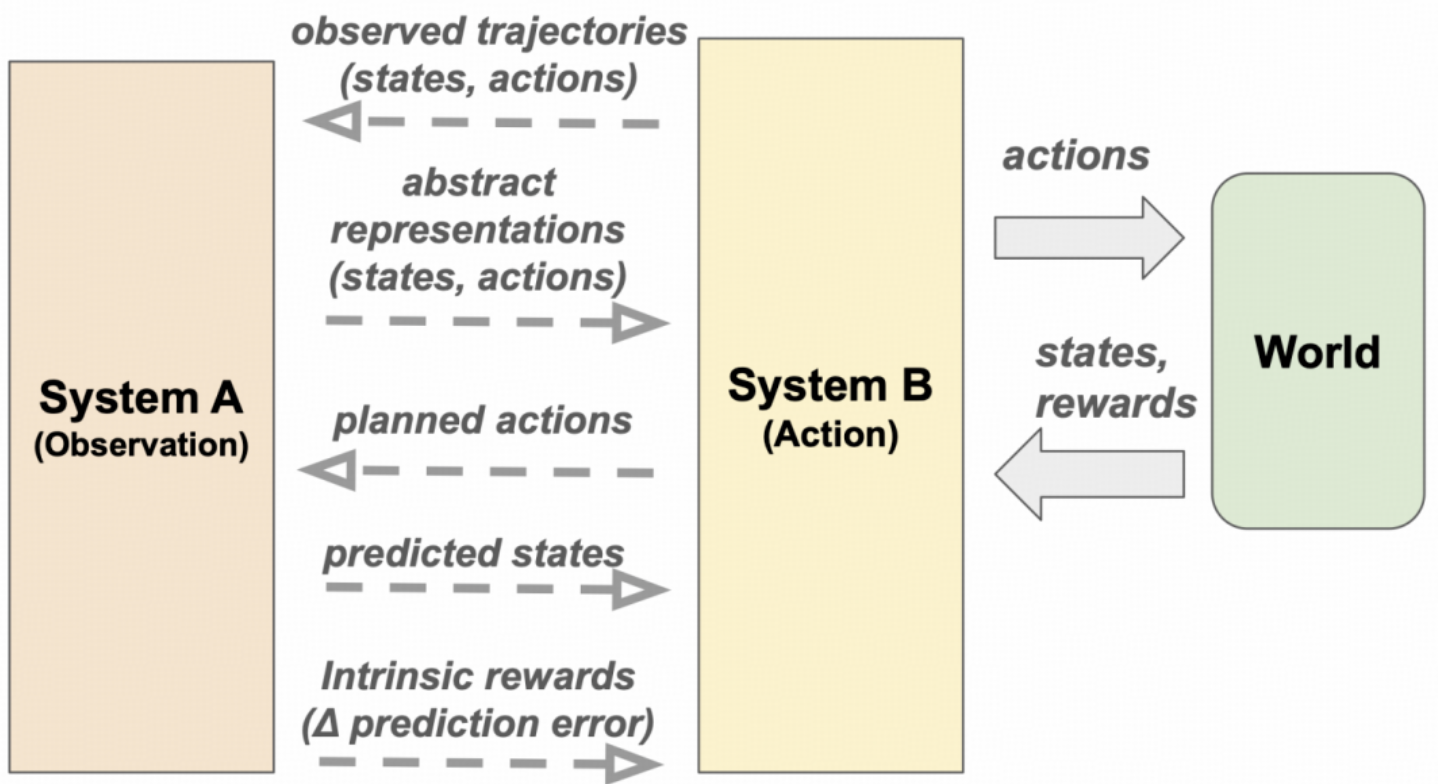
\includegraphics{images/image-0048.png}
\caption{A-B-M 自主学习架构示意图}
\end{figure}

\hypertarget{ux4e09ux53ccux5c42ux4f18ux5316}{%
\subsection{三、双层优化}\label{ux4e09ux53ccux5c42ux4f18ux5316}}

\textbf{内循环（发育尺度 Developmental Scale）}：这是单个智能体在其``一生''中的学习过程。利用给定的初始架构参数，系统 A 和系统 B 在固定的 System M 指挥下，与模拟环境实时交互、不断更新参数。

\textbf{外循环（演化尺度 Evolutionary Scale）}：在成千上万个模拟生命周期结束后，根据智能体是否完成了手工设计的生存适应度函数 \(\mathcal{L}\)，通过元学习算法去更新整个种群的``基因参数'' \(\phi\)。

数学形式化：

\[
\phi_{t+1} =
\arg\min_{\phi_t}
\mathcal{L}(A_0:A_K,B_0:B_K)
\]

这一优化必须受到开发育尺度的初始化和交互法则约束：

\[
A_0,B_0,M=\mathrm{Init}(\phi_t)
\]

\[
A_{i+1},B_{i+1}=\mathrm{Update}(M,A_i,B_i,Env)
\]

\hypertarget{ux56dbux9ad8ux7ea7ux5b66ux4e60ux5f62ux6001ux5c55ux671b}{%
\subsection{四、高级学习形态展望}\label{ux56dbux9ad8ux7ea7ux5b66ux4e60ux5f62ux6001ux5c55ux671b}}

在完善的元控制系统下，AI 有望展现出类似于大型哺乳动物和人类独有的高级学习形态：

\begin{itemize}
\tightlist
\item
  \textbf{通过沟通/社会化学习（Learning from Communication）}：System M 能够敏锐捕捉社会提示（如目光注视或教学语气），优先处理来自可靠来源（例如人类教师）的高优先级数据流，并快速同步给系统 A 建立新的世界规则。
\item
  \textbf{通过想象学习（Learning from Imagination）}：在休息甚至``睡眠''状态下，System M 能切断外部感官和运动输出，从情景记忆中提取经验进行高速回放，利用系统 A 在潜空间中推演长期计划，并在无需真实物理试错成本的情况下更新系统 B 的策略。
\end{itemize}

总结：这篇论文指出，想实现真正的通用人工智能并越过目前的数据墙，不应只依赖极度``语言中心化''且僵化的范式。AI 需要向认知科学取经，通过一个具有高度自决能力的元控制中心（System M），在``世界建模（观察）''和``具身控制（行动）''之间流畅切换，从而实现可以在部署后持续成长的自主生命体。

\hypertarget{ux53c2ux8003ux6587ux732e-153}{%
\subsection{参考文献}\label{ux53c2ux8003ux6587ux732e-153}}

\begin{itemize}
\tightlist
\item
  Dupoux, E., LeCun, Y., \& Malik, J. (2026). \href{https://arxiv.org/abs/2603.15381}{Why AI systems do not learn and what to do about it: Lessons on autonomous learning from cognitive science}. arXiv:2603.15381.
\end{itemize}

\clearpage
